% 第 5 章 可视化一、二、三形式
\chapter{可视化一、二、三形式}

在本章中，我们将引入并详细讨论物理学家有时用来可视化"良好"微分形式的一种方式. 本质上，我们将考虑在向量空间上可视化一形式、二形式与三形式的方法. 也就是说，我们将找到 $\alpha_p\in T_p^*\mathbb{R}^2$ 与 $\alpha_p\in T_p^*\mathbb{R}^3$ 的"漫画图". 我们对 $\alpha_p$ 的图将叠加在向量空间 $T_p\mathbb{R}^3$ 上. 这一视角在 Misner、Thorne 和 Wheeler 的巨著 \textit{Gravitation} 中得到了充分的发展. 事实上，他们也做出了一些努力来发展（时空的）四维图形，不过我们在这里将主要限于二维与三维的情形. 第 1 节集中讨论二维的情形，第 2 至第 4 节讨论三维的情形. 然后在第 5 节我们把我们的漫画图推广到一般的二维与三维流形. 再说一遍，这种漫画图实际上只适用于"良好"的微分形式，即物理学家更可能遇到的那种微分形式，但对于不太复杂的微分形式与流形，它仍然是有用的. 最后，在第 6 节我们引入 Hodge 星算子. 我们在三维中对形式的可视化提供了一种很好的方式来可视化 Hodge 星算子所做的事情，这使得这里成为引入它的好地方. 尽管本章发展的物理学中可视化微分形式的方式功能强大且有用，但它在数学中很少被遇到. 原因之一是，在现实中这并不是一种考虑形式的完全一般的方式；当处理大于四的维度、或更抽象的流形、或某种意义下不"良好"的形式时，它就不起作用了.

\section{R² 中的一形式与二形式}

我们从考虑一形式 $\alpha_p\in T_p^*\mathbb{R}^2$ 开始. 回忆一形式 $\alpha_p$ 在流形 $\mathbb{R}^2$ 的点 $p$ 处"吞入"向量 $v_p$. 我们将取点 $p$ 处的特定一形式 $dx_p$. 眼下我们在记号中暂时抑制 $p$，并假设一切发生在某一个特定的点 $p$ 处. 回忆一形式 $dx$ 是 0-形式 $x$ 的外微分，而 0-形式 $x$ 本身只不过就是坐标函数 $x$. 但在 0-形式的情形下，外微分就是函数的微分. 回忆函数 $f$ 的微分由 $df(v)=v[f]$ 定义，即 $f$ 在方向 $v$ 上的方向导数.

但是坐标函数 $x$ 在 $x$ 方向的变化率是多少呢？当然是 1. 换句话说，坐标函数 $x$ 的图像在 $x$ 方向的斜率是 1. 我们把斜率想成"rise"比"run"，即竖直变化除以水平变化. 但在定义方向导数时，我们对定义稍作调整，以容纳不是单位向量的向量. 方向导数给我们的不再是斜率，而是斜率的"rise"部分. 所以，对坐标函数 $x$，微分 $dx$ 度量发生在 $x$ 方向的"rise". 例如，考虑向量
\[
v=\binom{3}{2}.
\]
当一个人沿着向量 $v$ 从点 $(0,0)$ 移动到点 $(3,2)$ 时，坐标函数 $x$ 的图像"上升"了三个单位，因此
\[
dx\binom{3}{2}=3.
\]

\begin{question}\label{q:5-1}
画出 $\mathbb{R}^2$ 上的坐标函数 $x$，并求出坐标函数 $x$ 沿下列向量的"rise"：
\begin{enumerate}
  \item[(a)] $\binom{1}{0}$，即从点 $(0,0)$ 到点 $(1,0)$，
  \item[(b)] $\binom{-1}{0}$，即从点 $(0,0)$ 到点 $(-1,0)$，
  \item[(c)] $\binom{2}{2}$，即从点 $(0,0)$ 到点 $(2,2)$，
  \item[(d)] $\binom{-3}{-1}$，即从点 $(0,0)$ 到点 $(-3,-1)$.
\end{enumerate}
\end{question}

\begin{question}\label{q:5-2}
画出 $\mathbb{R}^2$ 上的坐标函数 $y$，并求出坐标函数 $y$ 沿下列向量的"rise"：
\begin{enumerate}
  \item[(a)] $\binom{0}{1}$，即从点 $(0,0)$ 到点 $(0,1)$，
  \item[(b)] $\binom{1}{1}$，即从点 $(0,0)$ 到点 $(1,1)$，
  \item[(c)] $\binom{-1}{2}$，即从点 $(0,0)$ 到点 $(-1,2)$，
  \item[(d)] $\binom{2}{-3}$，即从点 $(0,0)$ 到点 $(2,-3)$.
\end{enumerate}
\end{question}

这解释了我们最初引入一形式的方式. 我们引入一形式 $dx$ 的方式是把它作为 $v\in T_p\mathbb{R}^2$ 在 $T_p\mathbb{R}^2$ 的 $\frac{\partial}{\partial x}$ 轴上的投影. 这恰好就是坐标函数 $x$ 从点 $p$ 到 $v_p$ 的终点的"rise"量. 因此我们有
\begin{align*}
dx\binom{1}{4}=1,\quad dx\binom{-1}{4}=-1,\quad dx\binom{2}{5}=2,\quad dx\binom{3}{6}=3, \\
dx\binom{1}{2}=1,\quad dx\binom{-1}{3}=-1,\quad dx\binom{2}{2}=2,\quad dx\binom{3}{1}=3, \\
dx\binom{1}{-2}=1,\quad dx\binom{-1}{-2}=-1,\quad dx\binom{2}{-2}=2,\quad dx\binom{3}{-1}=3.
\end{align*}

考虑这如何在图~\ref{fig:5-1} 中说明. 由方程 $x=-1$、$x=0$、$x=1$、$x=2$、$x=3$ 等给出的竖直直线充当投影的图示. 例如，向量 $\binom{2}{5}$、$\binom{2}{2}$ 与 $\binom{2}{-2}$ 的终点都落在直线 $x=2$ 上. 于是这些向量中的每一个都"刺穿"了直线 $x=1$ 和 $x=2$. 如果一个向量的终点落在一条直线上，我们就认为该向量"刺穿"了这条直线. 我们不再把 $dx$ 想成向 $\frac{\partial}{\partial x}$ 轴上的投影，而是把 $dx$ 画成无穷序列的直线 $x=\pm n$，$n=0,1,2,3,\ldots$. 利用这幅图像，我们把 $dx(v)$ 解释为向量 $v$ 所刺穿的直线的条数.

\begin{figure}[htbp]
  \centering
  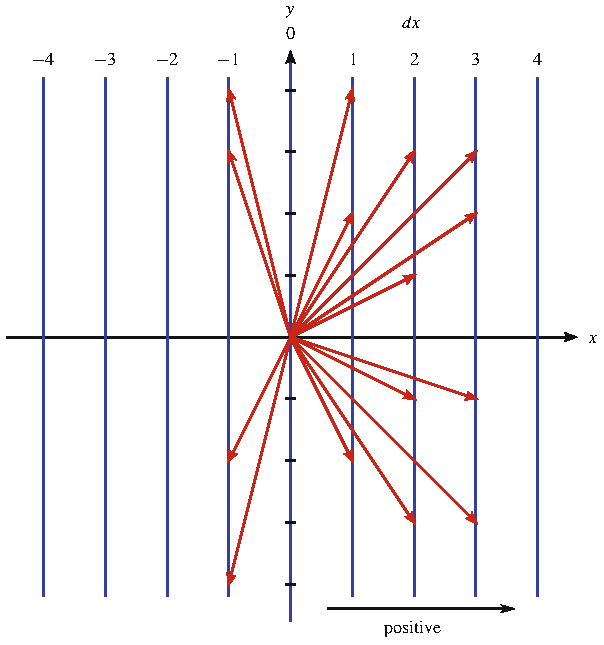
\includegraphics[width=0.716\linewidth]{images/vector/fig-5-1.pdf}
  \caption{使一形式 $dx$ 给出输出 $-1$、$1$、$2$ 和 $3$ 的向量. 图中显示了正方向}
  \label{fig:5-1}
\end{figure}

除了把 $dx$ 想成直线族 $x=\pm n$ 之外，我们还必须附上一个定向. 这在图中以指向右方的箭头显示，表示正定向. 于是向量 $\binom{-1}{4}$、$\binom{-1}{3}$ 与 $\binom{-1}{-2}$ 都刺穿一条直线，即直线 $x=-1$. 但由于这些向量是"向后"（沿负方向）走的，我们把它看作"刺穿负一次". 如果我们想考虑微分一形式 $-dx$，我们会得到同样的图，即由 $x=\pm n$ 给出的直线，但我们要把定向画在相反的方向.

现在考虑下面这些，
\begin{align*}
dx\binom{1.42}{4}=1.42,\quad dx\binom{1.97}{2}=1.97,\quad dx\binom{1.1}{-2}=1.1, \\
dx\binom{-1.21}{4}=-1.21,\quad dx\binom{-1.5}{3}=-1.5,\quad dx\binom{-1.92}{-2}=-1.92, \\
dx\binom{2.23}{5}=2.23,\quad dx\binom{2.74}{2}=2.74,\quad dx\binom{2.01}{-2}=2.01, \\
dx\binom{3.69}{6}=3.69,\quad dx\binom{3.91}{1}=3.91,\quad dx\binom{3.34}{-1}=3.34.
\end{align*}
显然 $dx\binom{1.42}{4}=1.42$ 是正确的，然而利用我们把 $dx$ 画成无穷序列直线 $x=\pm n$（$n=0,1,2,3,\ldots$）并附上定向的图像，向量 $\binom{1.42}{4.84}$ 只刺穿一条直线，即直线 $x=1$. 所以，利用关于 $dx$ 的"刺穿"图，我们有 $dx\binom{1.42}{4}=1$. 显然这不是精确的，但它的确给出一个近似. 利用这种刺穿的想法，我们会有
\begin{align*}
dx\binom{1.42}{4}=1,\quad dx\binom{1.97}{2}=1,\quad dx\binom{1.1}{-2}=1, \\
dx\binom{-1.21}{4}=-1,\quad dx\binom{-1.5}{3}=-1,\quad dx\binom{-1.92}{-2}=-1.
\end{align*}

以完全相同的方式，我们可以把微分形式 $dy_p\in T_p^*\mathbb{R}^2$ 表示成无穷序列的直线 $y=\pm n$（$n=0,1,2,3,\ldots$）连同定向，位于向量空间 $T_p\mathbb{R}^2$ 中. $dy_p(v_p)$ 的值是向量 $v_p$ 刺穿的直线的条数. 同样，如果向量的尖端碰到一条直线，即使它没有穿过这条直线，我们也认为它刺穿了这条直线.

\begin{figure}[htbp]
  \centering
  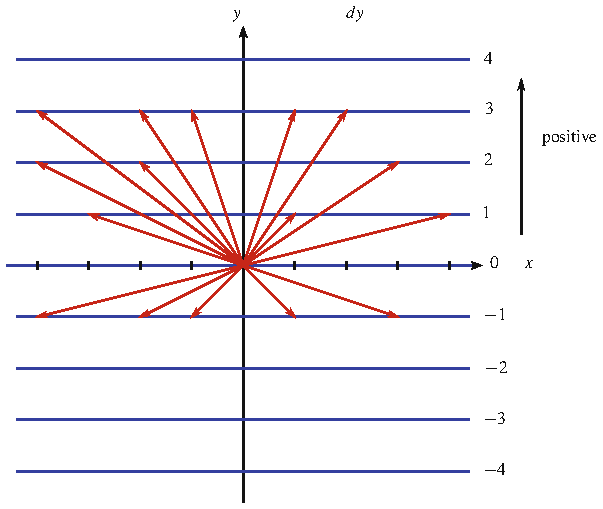
\includegraphics[width=0.715\linewidth]{images/vector/fig-5-2.pdf}
  \caption{使一形式 $dy$ 给出输出 $-1$、$1$、$2$ 和 $3$ 的向量. 图中显示了正方向}
  \label{fig:5-2}
\end{figure}

所以对于图~\ref{fig:5-2} 我们有
\begin{align*}
dy\binom{-2}{3}=3,\quad dy\binom{-2}{2}=2,\quad dy\binom{-3/2}{1}=1,\quad dy\binom{-2}{-1}=-1, \\
dy\binom{1}{3}=3,\quad dy\binom{1/2}{2}=2,\quad dy\binom{1}{1}=1,\quad dy\binom{-1}{-1}=-1, \\
dy\binom{4}{3}=3,\quad dy\binom{3}{2}=2,\quad dy\binom{3}{1}=1,\quad dy\binom{1}{-1}=-1.
\end{align*}
关于近似的上述评论同样适用. 例如，向量 $\binom{1.42}{4.84}$ 刺穿了我们的 $dy$ 图的四条直线，所以我们会得到 $dy\binom{1.42}{4.84}=4$，尽管精确值当然是 4.84.

但微分形式 $dx$ 与 $dy$ 并不是 $T_p^*\mathbb{R}^2$ 仅有的元素. 微分形式 $2dx_p\in T_p^*\mathbb{R}^2$ 在向量空间 $T_p\mathbb{R}^2$ 中会如何表示呢？考虑上面相同的向量，我们有
\begin{align*}
2dx\binom{1}{4}=2,\quad 2dx\binom{-1}{4}=-2,\quad 2dx\binom{2}{5}=4,\quad 2dx\binom{3}{6}=6, \\
2dx\binom{1}{2}=2,\quad 2dx\binom{-1}{3}=-2,\quad 2dx\binom{2}{2}=4,\quad 2dx\binom{3}{1}=6, \\
2dx\binom{1}{-2}=2,\quad 2dx\binom{-1}{-2}=-2,\quad 2dx\binom{2}{-2}=4,\quad 2dx\binom{3}{-1}=6.
\end{align*}

所以这些向量在 $2dx$ 的情形下刺穿的直线条数是 $dx$ 情形下的两倍，这意味着 $2dx$ 情形下直线的"密度"是 $dx$ 情形下直线的两倍. 我们会把它画成图~\ref{fig:5-3} 那样.

\begin{figure}[htbp]
  \centering
  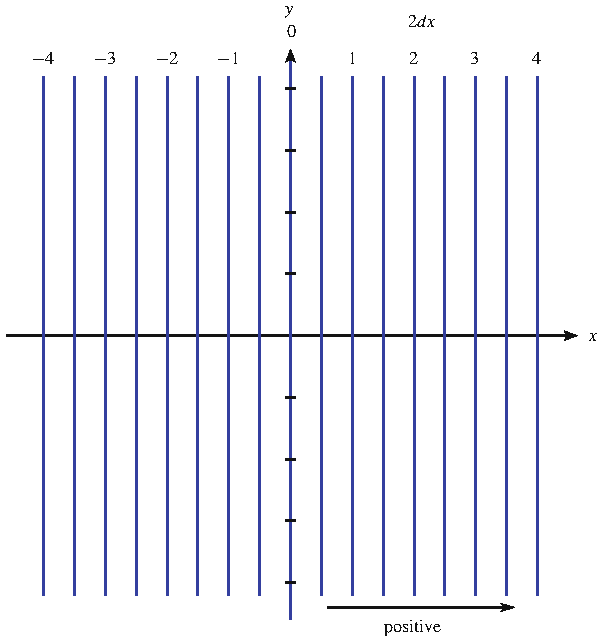
\includegraphics[width=0.716\linewidth]{images/vector/fig-5-3.pdf}
  \caption{用待刺穿的直线表示的一形式 $2dx$}
  \label{fig:5-3}
\end{figure}

我们可以在 $2dy$ 的情形下进行完全相同的分析. 同样，利用上面的相同向量，我们有
\begin{align*}
2dy\binom{-2}{3}=6,\quad 2dy\binom{-2}{2}=4,\quad 2dy\binom{-3/2}{1}=2,\quad 2dy\binom{-2}{-1}=-2, \\
2dy\binom{1}{3}=6,\quad 2dy\binom{1/2}{2}=4,\quad 2dy\binom{1}{1}=2,\quad 2dy\binom{-1}{-1}=-2, \\
2dy\binom{4}{3}=6,\quad 2dy\binom{3}{2}=4,\quad 2dy\binom{3}{1}=2,\quad 2dy\binom{1}{-1}=-2.
\end{align*}

同样，这些向量在 $2dy$ 的情形下刺穿的直线条数是 $dy$ 情形下的两倍，所以 $2dy$ 情形下直线的"密度"也是 $dy$ 情形下直线密度的两倍. 我们会把它画成图~\ref{fig:5-4} 那样.

\begin{figure}[htbp]
  \centering
  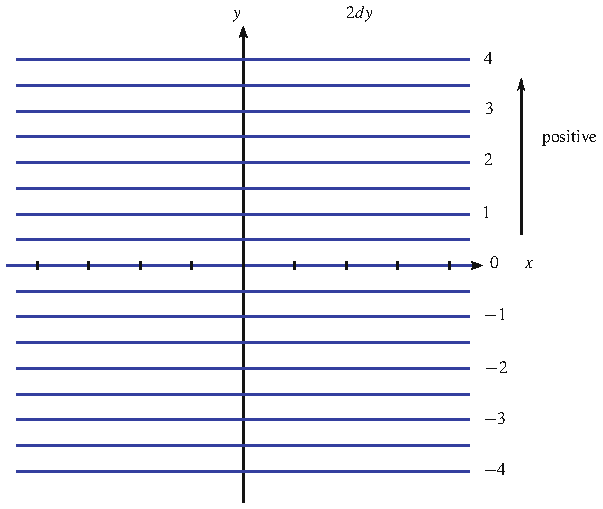
\includegraphics[width=0.715\linewidth]{images/vector/fig-5-4.pdf}
  \caption{用待刺穿的直线表示的一形式 $2dy$}
  \label{fig:5-4}
\end{figure}

显然，如果你对 $3dx$ 和 $3dy$ 做同样的分析，你会发现图形表示中直线的"密度"是 $dx$ 与 $dy$ 情形下的三倍，而对 $ndx$ 与 $ndy$ 则是 $n$ 倍.

\begin{question}\label{q:5-3}
画出表示下列微分形式的图：$3dx$、$5dy$、$\frac12dx$、$\frac23dx$、$\frac13dy$ 与 $\frac35dy$.
\end{question}

现在我们转向 $T_p^*\mathbb{R}^2$ 中更一般的元素. 我们从简单的东西 $dx+dy$ 开始. 考虑一形式 $dx+dy$ 如何作用在下列向量上，
\begin{align*}
(dx+dy)\binom{-1}{3}=-1+3=2,\qquad (dx+dy)\binom{1}{2}=1+2=3, \\
(dx+dy)\binom{-1}{1}=-1+1=0,\qquad (dx+dy)\binom{0}{1}=0+1=1, \\
(dx+dy)\binom{1}{1}=1+1=2,\qquad (dx+dy)\binom{-1}{0}=-1+0=-1, \\
(dx+dy)\binom{1}{0}=1+0=1,\qquad (dx+dy)\binom{0}{-1}=0-1=-1.
\end{align*}

图~\ref{fig:5-5} 是 $dx+dy$ 的一张可行的图. 它之所以可行，可以通过检查向量并数出它们刺穿了多少条直线（把所描绘的定向考虑进去）而看出来. 显然 $dx+dy$ 的图需要斜线. 通过检查可以明白，这些直线由 $y=-x+n$（$n=0,\pm1,\pm2,\ldots$）给出.

\begin{figure}[htbp]
  \centering
  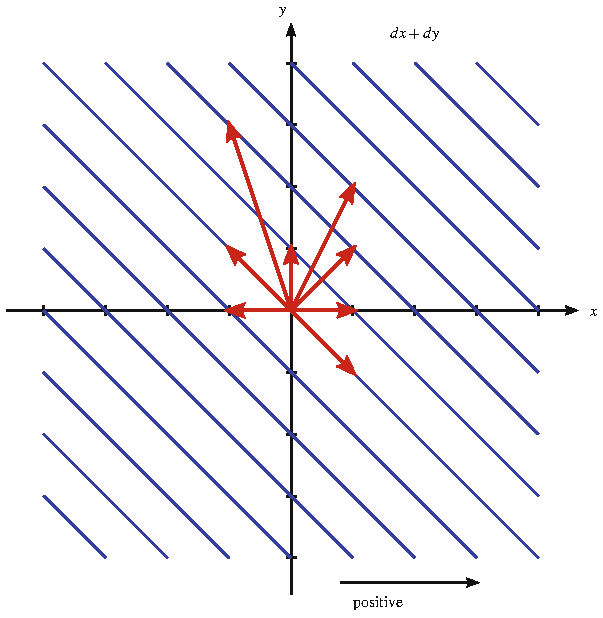
\includegraphics[width=0.715\linewidth]{images/vector/fig-5-5.pdf}
  \caption{一形式 $dx+dy$ 的待刺穿直线. 图中描绘了正方向}
  \label{fig:5-5}
\end{figure}

现在假设我们想画出微分一形式 $2dx+dy$、$dx-2dy$ 或更复杂的东西的图. 我们需要一种系统的方法来决定直线是什么. 这实际上相当容易. 考虑一形式 $2dx+dy$. 为了找到我们需要画出的直线来构成这个微分的图，我们只需从方程 $2x+y=n$（$n=0,\pm1,\pm2,\ldots$）开始，并解出 $y$，得到 $y=-2x+n$，如图~\ref{fig:5-6} 所示. 考虑图~\ref{fig:5-6} 中的向量 $v=\binom{1}{2}$. 它沿正方向"刺穿"了四条直线，所以根据图有 $(2dx+dy)(v)=4$. 计算上有
\[
(2dx+dy)\binom{1}{2}=2dx\binom{1}{2}+dy\binom{1}{2}=2(1)+2=4.
\]

类似地，为了画出一形式 $dx-2dy$ 的图，我们使用方程 $x-2y=n$，它变成 $y=\frac{x}{2}-\frac{n}{2}$. 见图~\ref{fig:5-7}.

\begin{figure}[htbp]
  \centering
  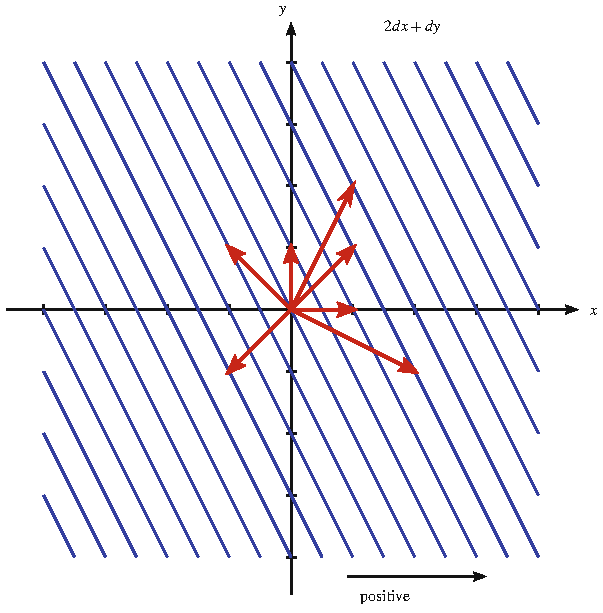
\includegraphics[width=0.715\linewidth]{images/vector/fig-5-6.pdf}
  \caption{一形式 $2dx+dy$ 的待刺穿直线. 图中描绘了正方向}
  \label{fig:5-6}
\end{figure}

\begin{figure}[htbp]
  \centering
  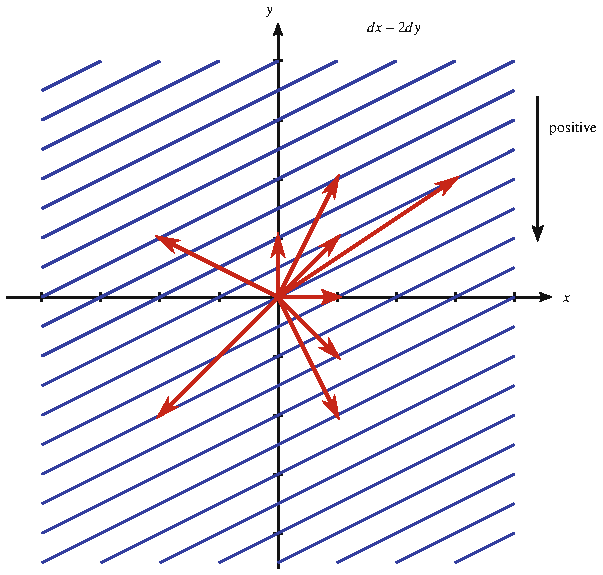
\includegraphics[width=0.742\linewidth]{images/vector/fig-5-7.pdf}
  \caption{一形式 $dx-2dy$ 的待刺穿直线. 图中描绘了正方向}
  \label{fig:5-7}
\end{figure}

\begin{question}\label{q:5-4}
检验在 $2dx+dy$ 与 $dx-2dy$ 的图中画出的各个向量，无论用计算还是用图形都给出相同的答案.
\end{question}

\begin{question}\label{q:5-5}
解释为什么上面寻找图形表示中直线的过程是可行的. 为此，考虑一般的一形式 $adx+bdy$ 如何作用在一般的向量 $v=\binom{x}{y}$ 上. 这个向量的哪些值给出 $(adx+bdy)(v)=n$（对任意 $n=0,\pm1,\pm2,\ldots$）？
\end{question}

\begin{question}\label{q:5-6}
画出下列微分形式的图形表示：
\begin{enumerate}
  \item[(a)] $3dx+dy$，
  \item[(b)] $2dx-dy$，
  \item[(c)] $-dx+3dy$.
\end{enumerate}
\end{question}

$T_p^*\mathbb{R}^2$ 中的微分一形式并不是唯一能作用在 $T_p\mathbb{R}^2$ 中向量上的形式. $\bigwedge_p^2(\mathbb{R}^2)$ 中的微分二形式也能作用在 $T_p\mathbb{R}^2$ 中的向量上. 如我们所知，微分二形式作用在 $T_p\mathbb{R}^2$ 中的两个向量上. 我们首先考虑向量
\[
v_1=\binom{1}{0},\qquad v_2=\binom{0}{1}
\]
以及微分二形式 $dx\wedge dy$. 我们有
\begin{align*}
(dx\wedge dy)(v_1,v_2)=
\begin{vmatrix}
dx(v_1) & dx(v_2)\\
dy(v_1) & dy(v_2)
\end{vmatrix}
=
\begin{vmatrix}
1 & 0\\
0 & 1
\end{vmatrix}
=1, \\
(dx\wedge dy)(v_2,v_1)=
\begin{vmatrix}
dx(v_2) & dx(v_1)\\
dy(v_2) & dy(v_1)
\end{vmatrix}
=
\begin{vmatrix}
0 & 1\\
1 & 0
\end{vmatrix}
=-1.
\end{align*}

和之前一样，我们想画一幅表示微分二形式 $dx\wedge dy$ 的 $T_p\mathbb{R}^2$ 中的图. 对微分一形式，我们使用由直线组成的图，然后数出我们的向量"刺穿"了多少条直线，从而得到该微分形式作用在向量上的近似值. 这里我们的图必须以某种方式把两个输入向量都考虑进去. 我们把 $T_p\mathbb{R}^2$ 中的微分二形式 $dx\wedge dy$ 表示为水平直线与竖直直线连同定向.

图~\ref{fig:5-8} 显示的是 $dx\wedge dy$ 的图，它由蓝色水平直线与绿色竖直直线组成，产生一个方形网格. 由向量 $v_1$ 与 $v_2$ 张成的平行六面体恰好覆盖网格的一个方格，因此我们说 $dx\wedge dy(v_1,v_2)$ 是 1. 现在我们只需要考虑定向. 由于 $(dx\wedge dy)(v_1,v_2)$ 是正的，我们用它来决定所需要的定向，这在图中被描绘为一个小圆形箭头，沿逆时针方向. 从 $v_1$ 到 $v_2$，沿着两个向量之间的最小角走过，是逆时针的，所以这就是被选择的定向. 因此，如果我们沿着第一个向量与第二个向量之间的最小角按逆时针方向走过，我们选择正；如果我们沿着第一个向量与第二个向量之间的最小角按顺时针方向走过，我们选择负. 所以对 $(dx\wedge dy)(v_2,v_1)$，第一个向量是 $v_2$，第二个向量是 $v_1$. 从第一个向量走到第二个向量，我们是沿顺时针方向走的，所以我们会选择负. 由向量 $v_2$ 与 $v_1$ 张成的平行六面体恰好覆盖一个方格，所以答案是 $-1$.

\begin{figure}[htbp]
  \centering
  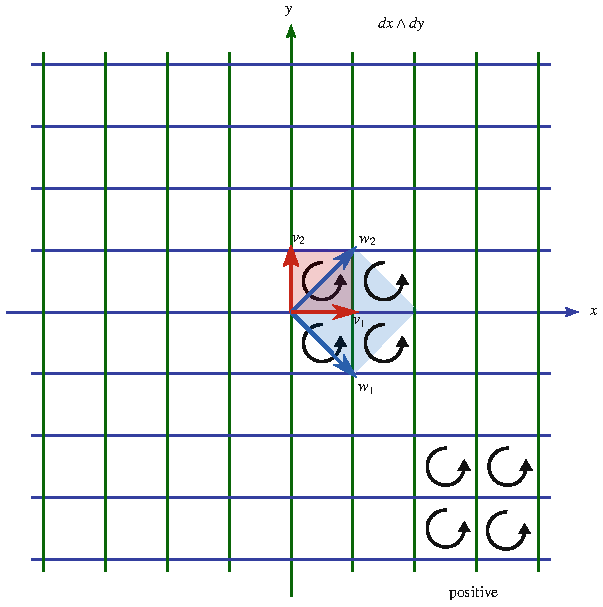
\includegraphics[width=0.715\linewidth]{images/vector/fig-5-8.pdf}
  \caption{二形式 $dx\wedge dy$ 由水平直线与竖直直线组成. 逆时针圆形箭头描绘了正方向}
  \label{fig:5-8}
\end{figure}

现在考虑向量
\[
w_1=\binom{1}{-1},\qquad w_2=\binom{1}{1}.
\]
计算上我们有
\begin{align*}
(dx\wedge dy)(w_1,w_2)=
\begin{vmatrix}
dx(w_1) & dx(w_2)\\
dy(w_1) & dy(w_2)
\end{vmatrix}
=
\begin{vmatrix}
1 & 1\\
-1 & 1
\end{vmatrix}
=2, \\
(dx\wedge dy)(w_2,w_1)=
\begin{vmatrix}
dx(w_2) & dx(w_1)\\
dy(w_2) & dy(w_1)
\end{vmatrix}
=
\begin{vmatrix}
1 & 1\\
1 & -1
\end{vmatrix}
=-2.
\end{align*}
利用图~\ref{fig:5-8} 可以看出，由 $w_1$ 与 $w_2$ 张成的平行六面体总共覆盖了两个网格方格，而如果我们沿最小角从 $w_1$ 走到 $w_2$，方向是逆时针的，所以我们选择正号，得到 $dx\wedge dy(w_1,w_2)=2$. 但如果我们沿最小角从 $w_2$ 走到 $w_1$，方向是顺时针的，所以我们选择负号，得到 $dx\wedge dy(w_2,w_1)=-2$.

现在我们转向微分二形式 $2dx\wedge dy$. 我们已经讨论过这种可视化微分形式的方式具有答案只是近似的缺点. 现在我们将说明另一个缺点. 对某些微分形式，我们使用什么样的图或图像可能有一些歧义. 我们再次考虑向量
\[
v_1=\binom{1}{0},\qquad v_2=\binom{0}{1},
\]
计算上它们给出
\[
(2dx\wedge dy)(v_1,v_2)=2
\begin{vmatrix}
1 & 0\\
0 & 1
\end{vmatrix}
=2.
\]
所以由 $v_1$ 与 $v_2$ 张成的平行六面体必须覆盖表示二形式 $2dx\wedge dy$ 的网格中的两个方框. 这样做的方式不是唯一的. 例如，对 $n=0,\pm1,\pm2,\ldots$ 选择直线 $y=n$ 与 $x=\frac{n}{2}$ 就能实现这一点；见图~\ref{fig:5-9}. 实现这一点的另一种方式是选择直线 $y=\frac{n}{2}$ 与 $x=n$（$n=0,\pm1,\pm2,\ldots$），如图~\ref{fig:5-10} 那样. 事实上，还有其他选择.

\begin{figure}[htbp]
  \centering
  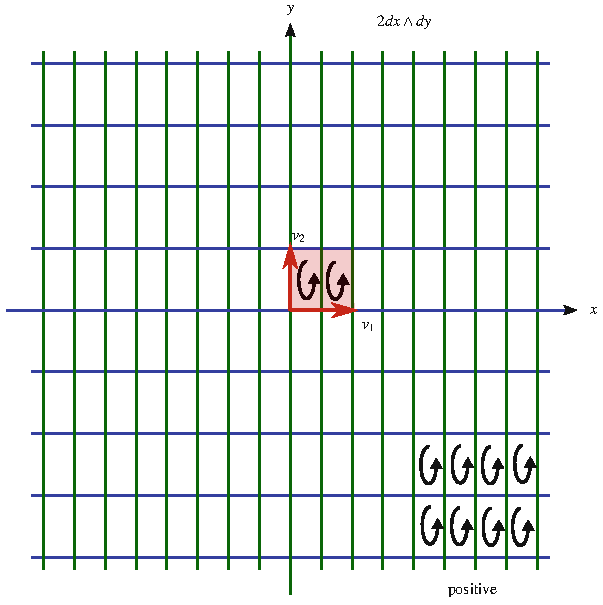
\includegraphics[width=0.715\linewidth]{images/vector/fig-5-9.pdf}
  \caption{画二形式 $2dx\wedge dy$ 的一种可行方式. 这里直线是 $x=n/2$ 与 $y=n$. 逆时针圆形箭头描绘了正方向}
  \label{fig:5-9}
\end{figure}

\begin{figure}[htbp]
  \centering
  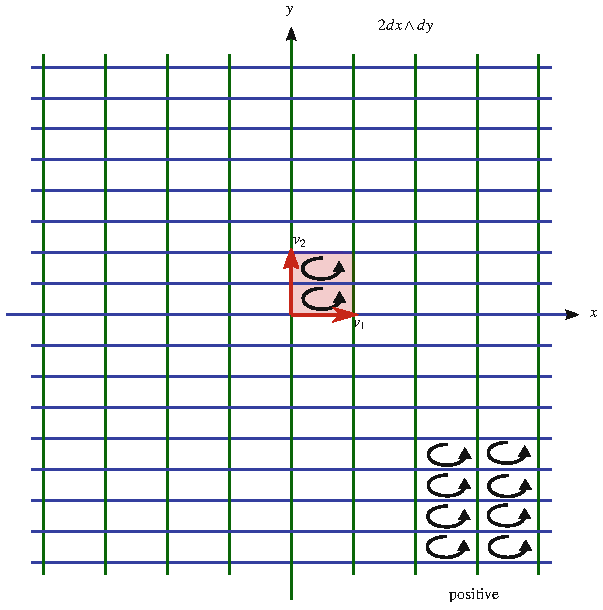
\includegraphics[width=0.715\linewidth]{images/vector/fig-5-10.pdf}
  \caption{画二形式 $2dx\wedge dy$ 的另一种可行方式. 这里直线是 $x=n$ 与 $y=n/2$. 逆时针圆形箭头描绘了正方向}
  \label{fig:5-10}
\end{figure}

\begin{question}\label{q:5-7}
为微分二形式 $2dx\wedge dy$ 找出另一种图形表示.
\end{question}

\begin{question}\label{q:5-8}
为下列每个微分二形式找出三种图形表示：
\begin{enumerate}
  \item[(a)] $3dx\wedge dy$，
  \item[(b)] $5dx\wedge dy$，
  \item[(c)] $\frac12dx\wedge dy$.
\end{enumerate}
\end{question}

\section{R³ 中的一形式}

和以前一样，我们固定流形 $\mathbb{R}^3$ 上的某一点 $p$，只考虑 $T_p^*\mathbb{R}^3$ 中的一形式. 我们将画出的一形式的"图"实际上叠加在向量空间 $T_p\mathbb{R}^3$ 上. 我们从一形式 $dx\in T_p^*\mathbb{R}^3$ 开始. 考虑 $dx$ 对下列向量的作用，
\begin{align*}
dx\begin{bmatrix}1\\0\\5\end{bmatrix}=1,\qquad
dx\begin{bmatrix}1\\0\\0\end{bmatrix}=1,\qquad
dx\begin{bmatrix}1\\2\\1\end{bmatrix}=1, \\
dx\begin{bmatrix}1\\2\\-1\end{bmatrix}=1,\qquad
dx\begin{bmatrix}1\\-3\\-2\end{bmatrix}=1,\qquad
dx\begin{bmatrix}1\\-4\\3\end{bmatrix}=1.
\end{align*}
任何终点落在 $T_p\mathbb{R}^3$ 中平面 $x=1$ 上的向量 $v\in T_p\mathbb{R}^3$ 都有值 1. 见图~\ref{fig:5-11}.

\begin{figure}[htbp]
  \centering
  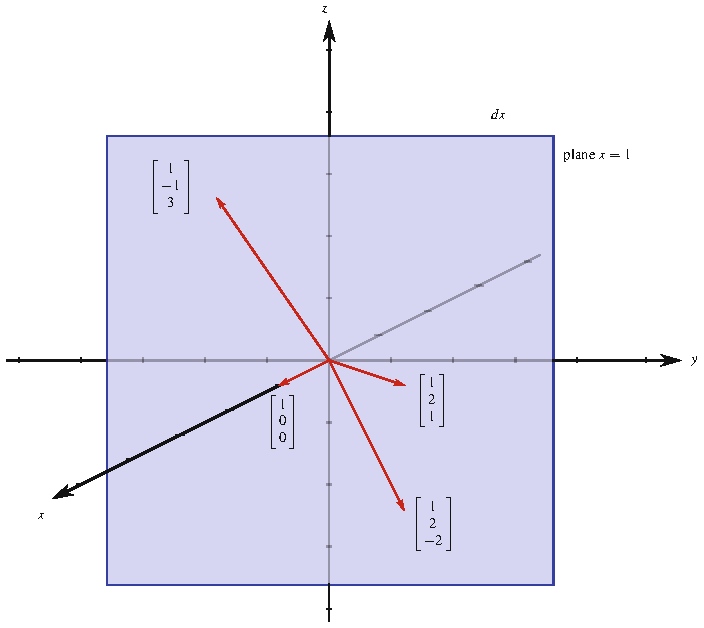
\includegraphics[width=0.891\linewidth]{images/vector/fig-5-11.pdf}
  \caption{$\mathbb{R}^3$ 中的平面 $x=1$. 一形式 $dx$ 把所有终点落在此平面上的向量送到值 1. 也就是说，若 $v$ 终点落在此平面上，则 $dx(v)=1$}
  \label{fig:5-11}
\end{figure}

类似地，考虑 $dx$ 对这些向量的作用，
\begin{align*}
dx\begin{bmatrix}3\\0\\0\end{bmatrix}=3,\qquad
dx\begin{bmatrix}2\\-2\\-1\end{bmatrix}=2,\qquad
dx\begin{bmatrix}0\\3\\4\end{bmatrix}=0, \\
dx\begin{bmatrix}3\\-1\\2\end{bmatrix}=3,\qquad
dx\begin{bmatrix}2\\-2\\-4\end{bmatrix}=2,\qquad
dx\begin{bmatrix}0\\-3\\-1\end{bmatrix}=0, \\
dx\begin{bmatrix}3\\2\\-5\end{bmatrix}=3,\qquad
dx\begin{bmatrix}2\\5\\-3\end{bmatrix}=2,\qquad
dx\begin{bmatrix}0\\-2\\5\end{bmatrix}=0.
\end{align*}

一形式把任何终点落在平面 $x=3$ 上的向量送到 $3$，把任何终点落在平面 $x=2$ 上的向量送到 $2$，把任何终点落在平面 $x=0$ 上的向量送到 $0$. 基于此，我们将在向量空间 $T_p\mathbb{R}^3$ 中把微分一形式 $dx\in T_p^*\mathbb{R}^3$ 图形化地表示为平面族 $x=n$，其中 $n=0,\pm1,\pm2,\ldots$. 在图~\ref{fig:5-12} 中，我们通过画出七个平面 $x=4$、$x=3$、$x=2$、$x=1$、$x=0$、$x=-1$ 与 $x=-2$ 来展示 $dx$.

\begin{figure}[htbp]
  \centering
  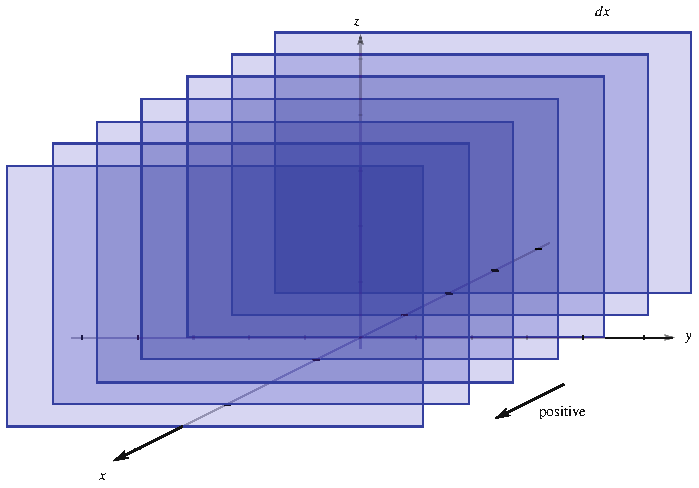
\includegraphics[width=0.863\linewidth]{images/vector/fig-5-12.pdf}
  \caption{在 $\mathbb{R}^3$ 中描绘为平面族的一形式 $dx$}
  \label{fig:5-12}
\end{figure}

利用这幅图我们说，向量 $v$ 的 $dx$ 就是 $v$ 所"刺穿"的平面的个数. 和以前一样，这样给出的答案只是近似答案. 例如，向量
\[
v_1=\begin{bmatrix}1\\-1\\7\end{bmatrix},\qquad
v_2=\begin{bmatrix}1.4\\1\\-2\end{bmatrix},\qquad
v_3=\begin{bmatrix}1.999\\-2\\5\end{bmatrix}
\]
都只刺穿一个平面，所以我们会说它们都有相同的值 $1$，尽管真正的答案显然是 $dx(v_1)=1$、$dx(v_2)=1.4$ 与 $dx(v_3)=1.999$. 同样，需要给这幅图赋予一个定向.

类似的推理得出，$dy$ 被图形化地表示为平面族 $y=n$，其中 $n=0,\pm1,\pm2,\ldots$，见图~\ref{fig:5-13}；而 $dz$ 被图形化地表示为平面族 $z=n$，其中 $n=0,\pm1,\pm2,\ldots$，见图~\ref{fig:5-14}.

\begin{figure}[htbp]
  \centering
  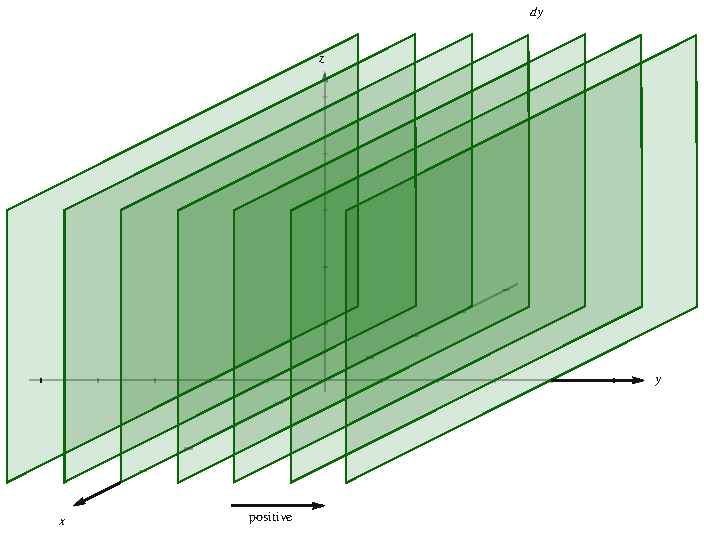
\includegraphics[width=0.947\linewidth]{images/vector/fig-5-13.pdf}
  \caption{在 $\mathbb{R}^3$ 中描绘为平面族的一形式 $dy$}
  \label{fig:5-13}
\end{figure}

\begin{figure}[htbp]
  \centering
  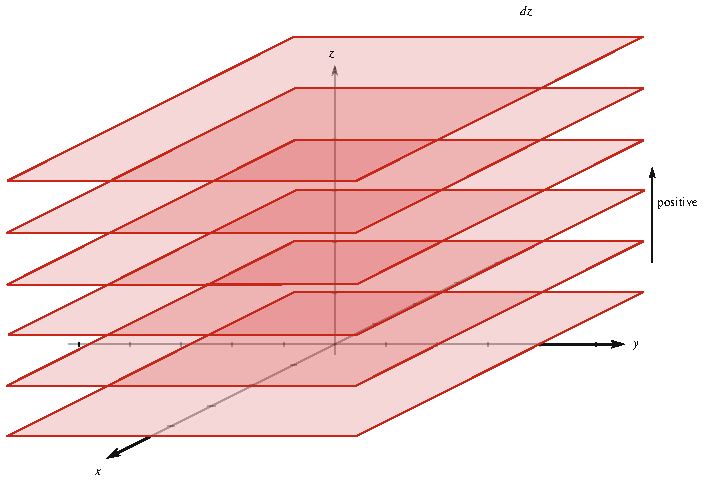
\includegraphics[width=0.960\linewidth]{images/vector/fig-5-14.pdf}
  \caption{在 $\mathbb{R}^3$ 中描绘为平面族的一形式 $dz$}
  \label{fig:5-14}
\end{figure}

\begin{question}\label{q:5-9}
证明图~\ref{fig:5-12}、图~\ref{fig:5-13} 与图~\ref{fig:5-14} 中描绘的正定向是正确的.
\end{question}

让我们花一点时间，把我们作为余切空间 $T_p^*\mathbb{R}^3$ 元素看待微分一形式的方式，与我们在 $T_p\mathbb{R}^3$ 上可视化微分形式的方式作一比较. 见图~\ref{fig:5-15}. $T_p^*\mathbb{R}^3$ 中的微分一形式也被称为余向量，它在余切空间中的画法与向量在切空间中的画法完全一样. 例如，一形式 $dx$ 是沿 $dx$ 轴的单位向量，一形式 $dy$ 是沿 $dy$ 轴的单位向量，一形式 $dz$ 是沿 $dz$ 轴的单位向量. 回忆我们选择总把余向量写成行向量，因此在 $T_p^*\mathbb{R}^3$ 中有 $dx=[1,0,0]$、$dy=[0,1,0]$、$dz=[0,0,1]$，所以一形式 $dx+dy+dz=[1,1,1]$. 在图~\ref{fig:5-15} 的上部，我们分别用蓝色、绿色与红色显示余向量 $dx$、$dy$ 与 $dz$.

\begin{figure}[htbp]
  \centering
  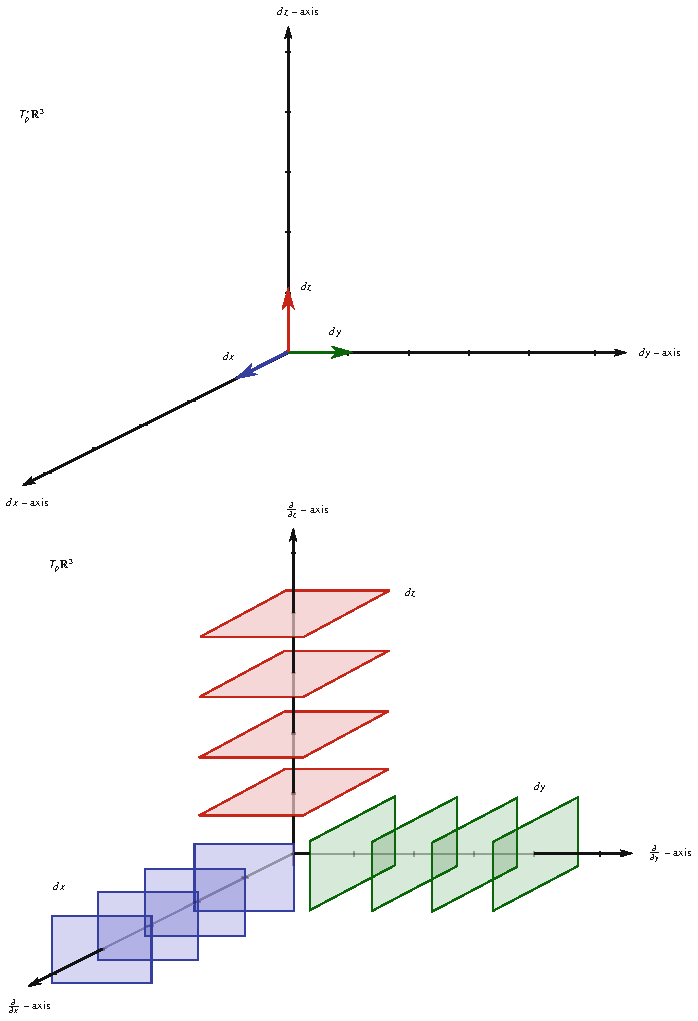
\includegraphics[width=0.852\linewidth]{images/vector/fig-5-15.pdf}
  \caption{一形式 $dx$（蓝）、$dy$（绿）与 $dz$（红）：上部在 $T_p^*\mathbb{R}^3$ 中描绘为余向量，下部在 $T_p\mathbb{R}^3$ 中描绘为平面}
  \label{fig:5-15}
\end{figure}

利用我们在本章引入的可视化微分形式的方法，微分一形式 $dx$ 被看成 $T_p\mathbb{R}^3$ 中垂直于 $\frac{\partial}{\partial x}$ 轴（也记为 $\frac{\partial}{\partial x}$ 轴）的无穷多个平面. 同样，微分一形式 $dy$ 是垂直于 $\frac{\partial}{\partial y}$ 轴的无穷多个平面，$dz$ 是垂直于 $\frac{\partial}{\partial z}$ 轴的无穷多个平面. 在图~\ref{fig:5-15} 的下部，我们分别用蓝色、绿色与红色显示了 $dx$、$dy$ 与 $dz$ 的少数几个平面.

与一形式 $dx$、$dy$、$dz$ 一样，一般的一形式 $adx+bdy+cdz$（其中 $a,b,c\in\mathbb{R}$）也可以被可视化为一族无穷多个平面. 作为例子，我们考虑一形式 $dx+dy$. 本质上，我们想以某种方式把 $dx$ 平面与 $dy$ 平面相加. 见图~\ref{fig:5-16}. 本质上，$dx$ 的平面垂直于向量
\[
\begin{bmatrix}1\\0\\0\end{bmatrix}
\]
而 $dy$ 的平面垂直于向量
\[
\begin{bmatrix}0\\1\\0\end{bmatrix}
\]
所以 $dx$ 与 $dy$ 的和，即 $dx+dy$，将是垂直于这两个向量之和的平面，也就是说，$dx+dy$ 的平面垂直于向量
\[
\begin{bmatrix}1\\1\\0\end{bmatrix}.
\]
答案显示在图~\ref{fig:5-17} 中.

\begin{figure}[htbp]
  \centering
  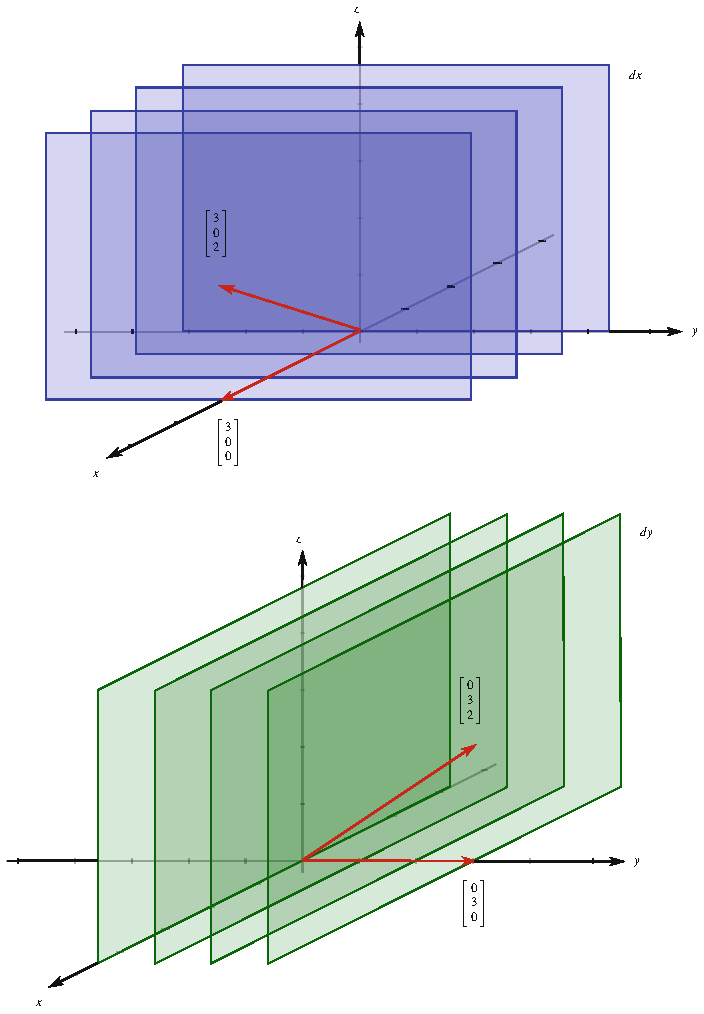
\includegraphics[width=0.865\linewidth]{images/vector/fig-5-16.pdf}
  \caption{为了找到 $dx+dy$ 的图形，我们想要以某种方式把 $dx$ 的平面（上）与 $dy$ 的平面（下）"相加". 这种"相加"给出图~\ref{fig:5-17} 中描绘的平面}
  \label{fig:5-16}
\end{figure}

\begin{figure}[htbp]
  \centering
  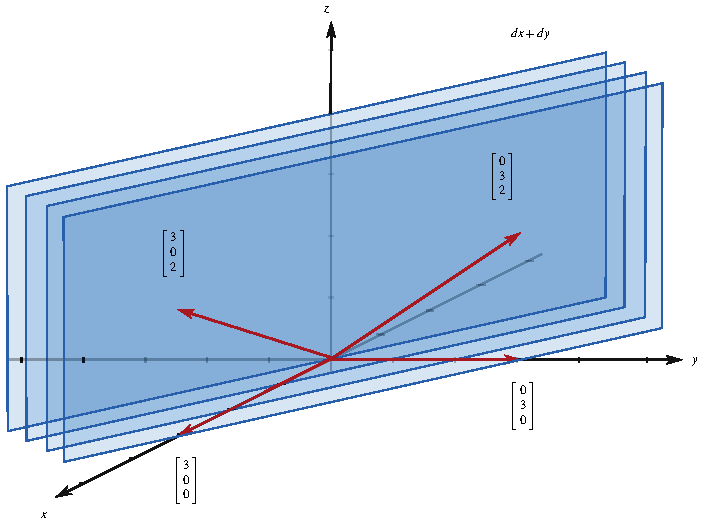
\includegraphics[width=0.960\linewidth]{images/vector/fig-5-17.pdf}
  \caption{描绘一形式 $dx+dy$ 的平面}
  \label{fig:5-17}
\end{figure}

Misner、Thorne 和 Wheeler 的书 \textit{Gravitation} 描述了寻找与 $dx+dy$ 相联系的平面的图形方法：选择适当的向量（比如下一个问题中的 $v_1$、$v_2$、$w_1$、$w_2$），数出它们刺穿的平面个数，然后用这些向量的端点来确定 $dx+dy$ 的一个平面. 下面几个问题将引导你走完他们的过程.

\begin{question}\label{q:5-10}
考虑向量
\[
v_1=\begin{bmatrix}3\\0\\0\end{bmatrix},\qquad
v_2=\begin{bmatrix}3\\0\\2\end{bmatrix},\qquad
w_1=\begin{bmatrix}0\\3\\0\end{bmatrix},\qquad
w_2=\begin{bmatrix}0\\3\\2\end{bmatrix}
\]
它们显示在图~\ref{fig:5-16} 中.
\begin{enumerate}
  \item[(a)] 分别用计算与图形从上面的图求出 $dx(v_1)$、$dx(v_2)$、$dx(w_1)$ 与 $dx(w_2)$.
  \item[(b)] 分别用计算与图形从上面的图求出 $dy(v_1)$、$dy(v_2)$、$dy(w_1)$ 与 $dy(w_2)$.
  \item[(c)] 分别用计算与图形从上面的图求出 $(dx+dy)(v_1)$、$(dx+dy)(v_2)$、$(dx+dy)(w_1)$ 与 $(dx+dy)(w_2)$.
  \item[(d)] $v_1$ 与 $v_2$ 刺穿了多少个 $dx$ 平面？多少个 $dy$ 平面？$w_1$ 与 $w_2$ 刺穿了多少个 $dy$ 平面？多少个 $dx$ 平面？那么这些向量中的每一个又刺穿多少个 $dx+dy$ 平面？
  \item[(e)] 基于 (a)--(d)，确定你将如何用向量 $v_1$、$v_2$、$w_1$、$w_2$ 来寻找 $dx+dy$ 的平面.
\end{enumerate}
\end{question}

\begin{question}\label{q:5-11}
在 $\mathbb{R}^3$ 上画出微分一形式 $dy+dz$ 与 $dx+dz$ 的草图.
\end{question}

现在我们有了比较 $dx+dy+dz$ 在 $T_p^*\mathbb{R}^3$ 中的表示与我们正在 $T_p\mathbb{R}^3$ 中可视化这一相同微分形式的方式所必需的全部构件，如图~\ref{fig:5-18} 那样.

\begin{figure}[htbp]
  \centering
  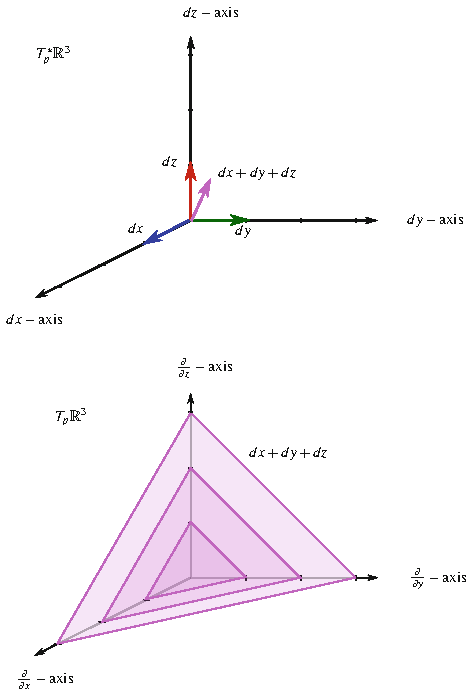
\includegraphics[width=0.573\linewidth]{images/vector/fig-5-18.pdf}
  \caption{一形式 $dx+dy+dz$：上部作为 $T_p^*\mathbb{R}^3$ 中的余向量，下部为在 $T_p\mathbb{R}^3$ 中描绘 $dx+dy+dz$ 的平面}
  \label{fig:5-18}
\end{figure}

\section{R³ 中的二形式}

类似于我们在 $T_p\mathbb{R}^2$ 中画二形式的方式，我们可以在 $T_p\mathbb{R}^3$ 中画二形式. 事实上，我们在 $T_p\mathbb{R}^3$ 中对二形式的图形表示本质上将是二维情形中网格线的三维版本. 我们不再尝试一步步走过这些图的推导过程，而是直接给出二形式 $dx\wedge dy$、$dy\wedge dz$ 与 $dz\wedge dx$ 的图，并说明它们是如何工作的. 我们从图~\ref{fig:5-19} 中二形式 $dx\wedge dy$ 的图开始.

\begin{figure}[htbp]
  \centering
  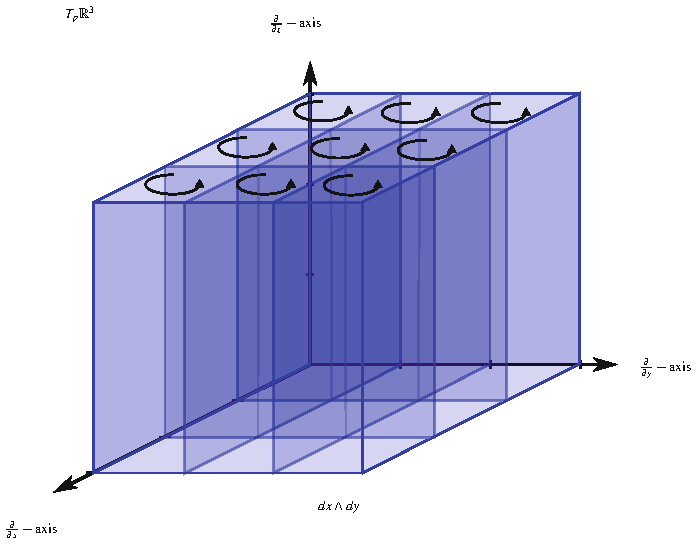
\includegraphics[width=0.960\linewidth]{images/vector/fig-5-19.pdf}
  \caption{在 $T_p\mathbb{R}^3$ 中描绘为一系列"管子"的二形式 $dx\wedge dy$，这些管子由平行于 $\frac{\partial}{\partial x}$ 轴与 $\frac{\partial}{\partial y}$ 轴的平面组成. 图中说明了正方向}
  \label{fig:5-19}
\end{figure}

注意，从图形上看，$dx\wedge dy$ 只不过就是同时画出 $dx$ 与 $dy$ 的平面，结果得到沿 $\frac{\partial}{\partial z}$ 方向延伸的"管子". 定向由管子中的小圆形箭头描绘. 俯视图上看，这些箭头沿逆时针方向转动. 我们不试图证明这是正确的图，而是用几个例子说明它是可行的. 首先考虑向量
\[
u_1=\begin{bmatrix}3\\0\\0\end{bmatrix}\qquad\text{与}\qquad u_2=\begin{bmatrix}0\\3\\0\end{bmatrix}.
\]
我们有
\[
(dx\wedge dy)(u_1,u_2)=
\begin{vmatrix}
3 & 0\\
0 & 3
\end{vmatrix}
=9.
\]
通过想象把向量 $u_1$ 与 $u_2$ 叠加到图~\ref{fig:5-19} 上，你可以看到由它们张成的平行六面体有九个 $dx\wedge dy$ 的"管子"穿过. 而且，当我们沿两个向量之间的最小角从 $u_1$ 走到 $u_2$ 时，我们移动的方向与施加在管子上的定向一致，所以这个 9 是正的. 如果我们沿两个向量之间的最小角从 $u_2$ 走到 $u_1$，那么我们移动的方向与施加在管子上的定向相反，所以在这种情形下 9 是负的，正如我们从计算
\[
(dx\wedge dy)(u_2,u_1)=
\begin{vmatrix}
0 & 3\\
3 & 0
\end{vmatrix}
=-9
\]
所预期的那样.

现在想象向量
\[
v_1=\begin{bmatrix}3\\0\\0\end{bmatrix}\qquad\text{与}\qquad v_2=\begin{bmatrix}0\\0\\3\end{bmatrix}
\]
叠加到图~\ref{fig:5-19} 上. 由这两个向量张成的平行六面体与管子平行，因而不穿过任何管子，所以在图形上我们有 $dx\wedge dy(v_1,v_2)=0$. 计算上我们得到相同的结果：
\[
(dx\wedge dy)(v_1,v_2)=
\begin{vmatrix}
3 & 0\\
0 & 0
\end{vmatrix}
=0.
\]

最后，想象向量
\[
w_1=\begin{bmatrix}0\\3\\0\end{bmatrix}\qquad\text{与}\qquad w_2=\begin{bmatrix}0\\0\\3\end{bmatrix}
\]
叠加到图~\ref{fig:5-19} 上. 同样，由 $w_1$ 与 $w_2$ 张成的平行六面体与管子平行，因而不穿过其中任何一根，给出 $dx\wedge dy(w_1,w_2)=0$，这同样与计算
\[
(dx\wedge dy)(w_1,w_2)=
\begin{vmatrix}
0 & 0\\
3 & 0
\end{vmatrix}
=0
\]
相符.

$dy\wedge dz$ 的图形表示与 $dx\wedge dy$ 非常相似，基本上由 $dy$ 与 $dz$ 的平面组成，得到平行于 $\frac{\partial}{\partial x}$ 轴的管子，如图~\ref{fig:5-20} 那样. 我们再次考虑由 $u_1$ 与 $u_2$、$v_1$ 与 $v_2$、$w_1$ 与 $w_2$ 张成的平行六面体与多少根管子相交. 计算上我们有
\begin{align*}
(dy\wedge dz)(u_1,u_2)=
\begin{vmatrix}
0 & 3\\
0 & 0
\end{vmatrix}
=0, \\
(dy\wedge dz)(v_1,v_2)=
\begin{vmatrix}
0 & 0\\
0 & 3
\end{vmatrix}
=0, \\
(dy\wedge dz)(w_1,w_2)=
\begin{vmatrix}
3 & 0\\
0 & 3
\end{vmatrix}
=9.
\end{align*}

\begin{figure}[htbp]
  \centering
  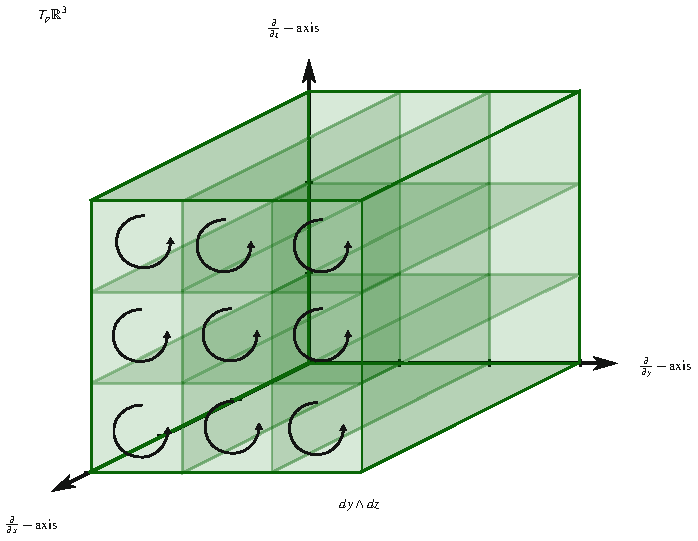
\includegraphics[width=0.960\linewidth]{images/vector/fig-5-20.pdf}
  \caption{在 $T_p\mathbb{R}^3$ 中描绘为一系列"管子"的二形式 $dy\wedge dz$，这些管子由平行于 $\frac{\partial}{\partial y}$ 轴与 $\frac{\partial}{\partial z}$ 轴的平面组成. 图中说明了正方向}
  \label{fig:5-20}
\end{figure}

通过想象把向量 $u_1$ 与 $u_2$ 叠加到 $dy\wedge dz$ 的图上，我们可以看到由这两个向量张成的平行六面体与管子平行，因而不穿过其中任何一根. 类似地，由 $v_1$ 与 $v_2$ 张成的平行六面体不穿过任何管子，但由 $w_1$ 与 $w_2$ 张成的平行六面体穿过九根管子.

最后，$dz\wedge dx$ 的图形表示由 $dz$ 与 $dx$ 的平面组成，得到平行于 $\frac{\partial}{\partial y}$ 轴的管子. 见图~\ref{fig:5-21}. 用上面的向量做类似的分析会得到预期的结果.

\begin{figure}[htbp]
  \centering
  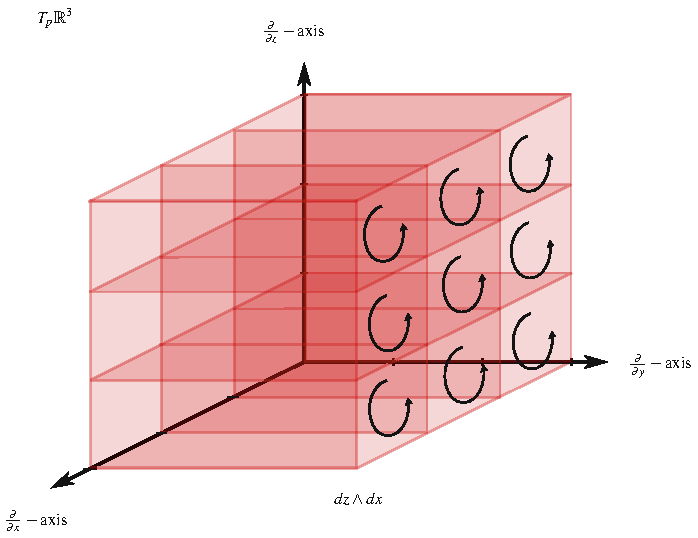
\includegraphics[width=0.887\linewidth]{images/vector/fig-5-21.pdf}
  \caption{在 $T_p\mathbb{R}^3$ 中描绘为一系列"管子"的二形式 $dz\wedge dx$，这些管子由平行于 $\frac{\partial}{\partial z}$ 轴与 $\frac{\partial}{\partial x}$ 轴的平面组成. 图中说明了正方向}
  \label{fig:5-21}
\end{figure}

当为二形式 $adx\wedge dy$、$bdy\wedge dz$、$cdz\wedge dx$（其中 $a,b,c\in\mathbb{R}$）寻找图形表示时，我们有与二维情形完全相同的歧义.

\begin{question}\label{q:5-12}
为微分二形式 $4dx\wedge dy$ 找出至少三种不同的图形表示.
\end{question}

现在我们考虑一般的微分二形式 $adx\wedge dy+bdy\wedge dz+cdz\wedge dx$，其中 $a,b,c\in\mathbb{R}$. 为简单起见，我们首先考虑二形式 $dx\wedge dy+dy\wedge dz$. 本质上，我们想找到这两幅图之和的图形表示，见图~\ref{fig:5-22}. 微分二形式 $dx\wedge dy$ 的管子平行于 $\frac{\partial}{\partial z}$ 轴，微分二形式 $dy\wedge dz$ 的管子平行于 $\frac{\partial}{\partial x}$ 轴. 考虑 $\frac{\partial}{\partial x}$ 方向的单位向量与 $\frac{\partial}{\partial z}$ 方向的单位向量. 把这两个单位向量相加，我们得到
\[
\begin{bmatrix}1\\0\\0\end{bmatrix}+\begin{bmatrix}0\\0\\1\end{bmatrix}=\begin{bmatrix}1\\0\\1\end{bmatrix}.
\]
$dx\wedge dy+dy\wedge dz$ 的管子平行于由这个向量确定的直线，如图~\ref{fig:5-23} 所示.

\begin{figure}[htbp]
  \centering
  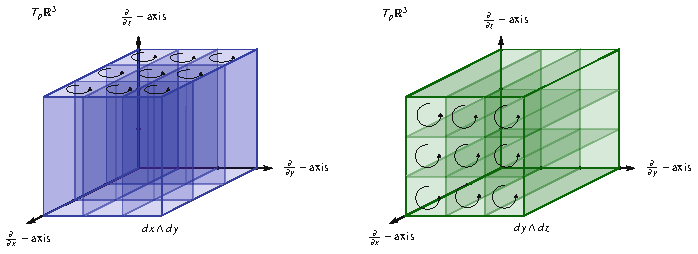
\includegraphics[width=0.960\linewidth]{images/vector/fig-5-22.pdf}
  \caption{为了找到二形式 $dx\wedge dy+dy\wedge dz$ 的图形表示，我们必须以某种方式把 $dx\wedge dy$（左）的管子与 $dy\wedge dz$（右）的管子"相加". 这些管子的"相加"结果如图~\ref{fig:5-23} 所示}
  \label{fig:5-22}
\end{figure}

\begin{figure}[htbp]
  \centering
  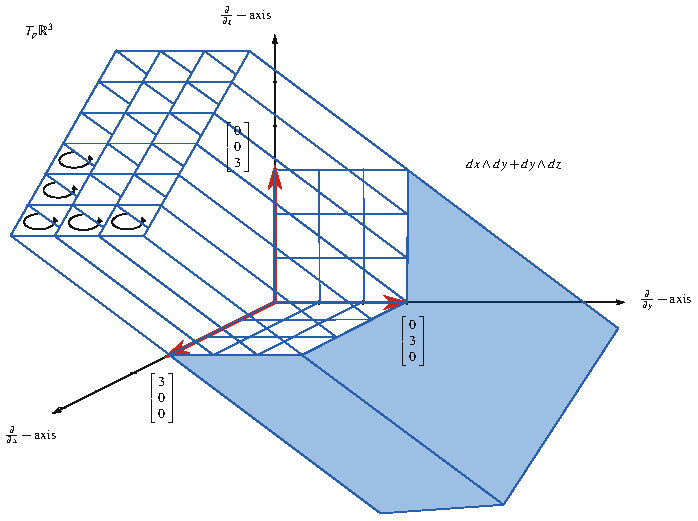
\includegraphics[width=0.940\linewidth]{images/vector/fig-5-23.pdf}
  \caption{把图~\ref{fig:5-22} 中 $dx\wedge dy$ 与 $dy\wedge dz$ 的管子"相加"所得的二形式 $dx\wedge dy+dy\wedge dz$ 的图形表示}
  \label{fig:5-23}
\end{figure}

\begin{question}\label{q:5-13}
设
\[
u=\begin{bmatrix}3\\0\\0\end{bmatrix},\qquad
v=\begin{bmatrix}0\\3\\0\end{bmatrix},\qquad
w=\begin{bmatrix}0\\0\\3\end{bmatrix}.
\]
借助图~\ref{fig:5-23} 证明，对下列各式，图形给出的答案与计算给出的答案一致：
\begin{enumerate}
  \item[(a)] $(dx\wedge dy+dy\wedge dz)(u,v)$，
  \item[(b)] $(dx\wedge dy+dy\wedge dz)(v,w)$，
  \item[(c)] $(dx\wedge dy+dy\wedge dz)(w,u)$.
\end{enumerate}
\end{question}

直观上看，与 $dx\wedge dy+dy\wedge dz$ 相联系的图似乎是有道理的. 还有另一种方式来看正在发生的事情. 回忆用来描绘一形式 $dx$ 的平面垂直于 $x$（或 $\frac{\partial}{\partial x}$）轴，用来描绘 $dy$ 的平面垂直于 $y$（或 $\frac{\partial}{\partial y}$）轴. 然后我们通过同时描绘这两族平面找到了 $dx\wedge dy$ 的图像. 我们的目标是把二形式 $dx\wedge dy+dy\wedge dz$ 变形为一种允许我们做类似事情的形式，
\[
dx\wedge dy+dy\wedge dz=-dy\wedge dx+dy\wedge dz=dy\wedge(-dx+dz)=dy\wedge d(-x+z).
\]

\begin{figure}[htbp]
  \centering
  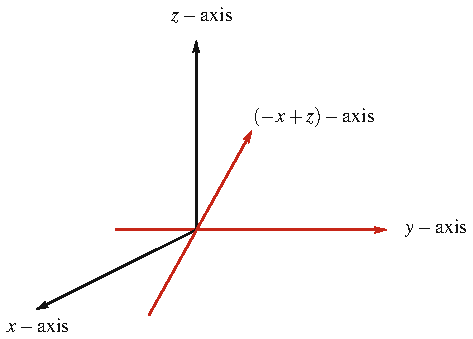
\includegraphics[width=0.561\linewidth]{images/vector/fig-5-24.pdf}
  \caption{垂直于 $y$ 轴与 $(-x+z)$ 轴的平面给出图~\ref{fig:5-23} 中所描绘的二形式 $dx\wedge dy+dy\wedge dz$}
  \label{fig:5-24}
\end{figure}

所以 $dx\wedge dy+dy\wedge dz$ 可以用垂直于 $y$ 轴与 $(-x+z)$"轴"的平面来表示. 最后这一点需要稍作解释. 考虑 $x$ 方向与 $z$ 方向的单位向量，把第一个的负向量加到第二个上，我们得到
\[
-\begin{bmatrix}1\\0\\0\end{bmatrix}+\begin{bmatrix}0\\0\\1\end{bmatrix}=\begin{bmatrix}-1\\0\\1\end{bmatrix}.
\]
向量 $\begin{bmatrix}-1\\0\\1\end{bmatrix}$ 确定了所使用的轴. 垂直于这个轴的平面是我们使用的第二族平面. 总之，对 $dx\wedge dy+dy\wedge dz$，使用的是垂直于图~\ref{fig:5-24} 中所画的两条红色轴的平面.

现在我们想找到 $dy\wedge dz+dz\wedge dx$ 的图，见图~\ref{fig:5-25}. 通过检查 $dy\wedge dz$ 与 $dz\wedge dx$ 的图可以看出，$dy\wedge dz+dz\wedge dx$ 的管子将平行于向量
\[
\begin{bmatrix}1\\1\\0\end{bmatrix}.
\]
或者我们也可以像前面那样改写 $dy\wedge dz+dz\wedge dx$，
\[
dy\wedge dz+dz\wedge dx=-dz\wedge dy+dz\wedge dx=dz\wedge(-dy+dx)=dz\wedge d(-y+x),
\]
并使用垂直于 $z$ 轴与 $(-y+x)$"轴"的平面，后者位于向量
\[
\begin{bmatrix}-1\\1\\0\end{bmatrix}
\]
的方向上. 这两个轴在图~\ref{fig:5-26} 中以红色显示.

\begin{figure}[htbp]
  \centering
  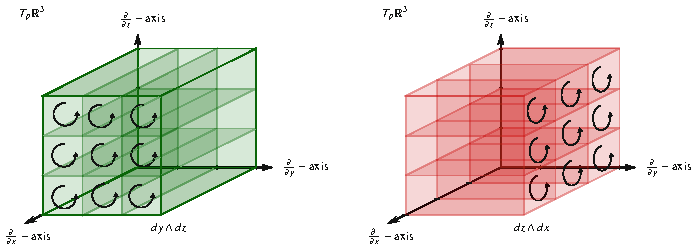
\includegraphics[width=0.960\linewidth]{images/vector/fig-5-25.pdf}
  \caption{为了找到二形式 $dy\wedge dz+dz\wedge dx$ 的图形表示，我们需要把 $dy\wedge dz$（左）与 $dz\wedge dx$（右）的管子"相加"}
  \label{fig:5-25}
\end{figure}

\begin{figure}[htbp]
  \centering
  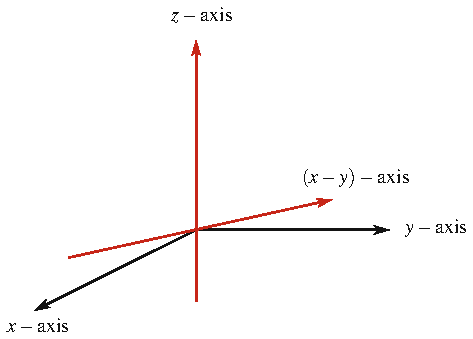
\includegraphics[width=0.561\linewidth]{images/vector/fig-5-26.pdf}
  \caption{$dy\wedge dz+dz\wedge dx$ 的管子由垂直于 $x$ 轴与 $(x-y)$ 轴的平面组成}
  \label{fig:5-26}
\end{figure}

现在我们想找到 $dx\wedge dy+dz\wedge dx$ 的图. 见图~\ref{fig:5-27}. 通过检查可以看出，$dx\wedge dy+dz\wedge dx$ 的管子平行于向量
\[
\begin{bmatrix}0\\1\\1\end{bmatrix},
\]
或者我们可以改写这个二形式，
\[
dx\wedge dy+dz\wedge dx=dx\wedge dy-dx\wedge dz=dx\wedge(dy-dz)=dx\wedge d(y-z)
\]
得到用来寻找垂直平面的两个轴. 这两个轴在图~\ref{fig:5-28} 中以红色显示.

\begin{figure}[htbp]
  \centering
  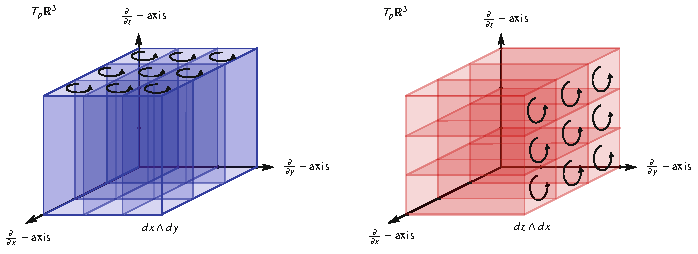
\includegraphics[width=0.960\linewidth]{images/vector/fig-5-27.pdf}
  \caption{二形式 $dx\wedge dy+dz\wedge dx$ 由把 $dx\wedge dy$（左）的管子与 $dz\wedge dx$（右）的管子相加得到}
  \label{fig:5-27}
\end{figure}

\begin{figure}[htbp]
  \centering
  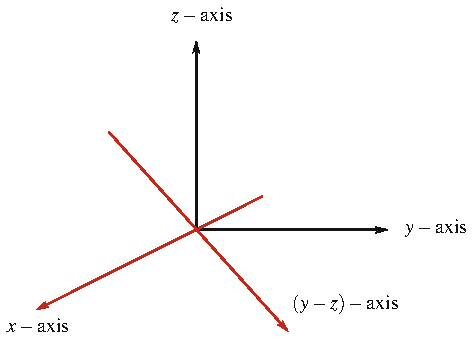
\includegraphics[width=0.561\linewidth]{images/vector/fig-5-28.pdf}
  \caption{二形式 $dx\wedge dy+dz\wedge dx$ 由垂直于 $x$ 轴与 $(y-z)$ 轴的平面组成}
  \label{fig:5-28}
\end{figure}

最后，我们想找到 $dx\wedge dy+dy\wedge dz+dz\wedge dx$ 的图. 见图~\ref{fig:5-29}. 我们可以如下改写二形式 $dx\wedge dy+dy\wedge dz+dz\wedge dx$，
\begin{align*}
dx\wedge dy+dy\wedge dz+dz\wedge dx=dy\wedge d(-x+z)+dz\wedge dx, \\
=dy\wedge d(-x+z)-dz\wedge(-dx)+dz\wedge dz, \\
=dy\wedge d(-x+z)-dz\wedge(-dx+dz), \\
=dy\wedge d(-x+z)-dz\wedge d(-x+z), \\
=(dy-dz)\wedge d(-x+z), \\
=d(y-z)\wedge d(-x+z),
\end{align*}
它可以用来勾画这个二形式. 最后，当转向带系数的二形式时，所有常见的问题都会出现.

\begin{figure}[htbp]
  \centering
  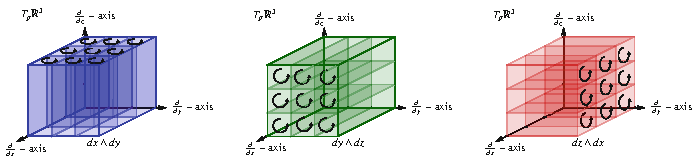
\includegraphics[width=0.960\linewidth]{images/vector/fig-5-29.pdf}
  \caption{二形式 $dx\wedge dy+dy\wedge dz+dz\wedge dx$ 由"相加"$dx\wedge dy$（左）、$dy\wedge dz$（中）与 $dz\wedge dx$（右）的管子得到}
  \label{fig:5-29}
\end{figure}

\begin{question}\label{q:5-14}
画出二形式 $dy\wedge dz+dz\wedge dx$ 的草图.
\end{question}

\begin{question}\label{q:5-15}
画出二形式 $dx\wedge dy+dz\wedge dx$ 的草图.
\end{question}

\begin{question}\label{q:5-16}
画出二形式 $dx\wedge dy+dy\wedge dz+dz\wedge dx$ 的草图.
\end{question}

\begin{question}\label{q:5-17}
画出下列每个二形式的一幅草图：
\begin{enumerate}
  \item[(a)] $2dx\wedge dy+dy\wedge dz$，
  \item[(b)] $dx\wedge dy+3dy\wedge dz$，
  \item[(c)] $2dx\wedge dy+4dy\wedge dz$.
\end{enumerate}
\end{question}

\begin{question}\label{q:5-18}
画出下列每个二形式的一幅草图：
\begin{enumerate}
  \item[(a)] $3dy\wedge dz+2dz\wedge dx$，
  \item[(b)] $dx\wedge dy+3dz\wedge dx$，
  \item[(c)] $2dx\wedge dy+4dy\wedge dz+3dz\wedge dx$.
\end{enumerate}
\end{question}

\begin{question}\label{q:5-19}
画出下列二形式的草图：
\begin{enumerate}
  \item[(a)] $-dx\wedge dy+dy\wedge dz$，
  \item[(b)] $dx\wedge dy-dy\wedge dz$，
  \item[(c)] $-dx\wedge dy-dy\wedge dz$.
\end{enumerate}
负号有什么影响？用一些精心选择的向量来帮助你弄清楚.
\end{question}

\section{R³ 中的三形式}

这很可能是整本书中最短的一节. 这是有原因的. 在 $T_p\mathbb{R}^3$ 中画三形式事实上极其简单. $\mathbb{R}^3$ 上的三形式空间，记为 $\bigwedge^3(\mathbb{R}^3)$，实际上是一维的，这意味着 $\mathbb{R}^3$ 上的每个三形式都有 $cdx\wedge dy\wedge dz$ 的形式，其中 $c\in\mathbb{R}$. 一形式 $dx$ 由平面 $x=n$ 给出，一形式 $dy$ 由平面 $y=n$ 给出，一形式 $dz$ 由平面 $z=n$ 给出，其中 $n=0,\pm1,\pm2,\ldots$. 三形式只不过就是同时画出所有这些平面，从而用单位立方体填满空间. 见图~\ref{fig:5-30}. 对于三形式 $adx\wedge dy\wedge dz$（其中 $a\in\mathbb{R}$），会出现常见的歧义.

\begin{figure}[htbp]
  \centering
  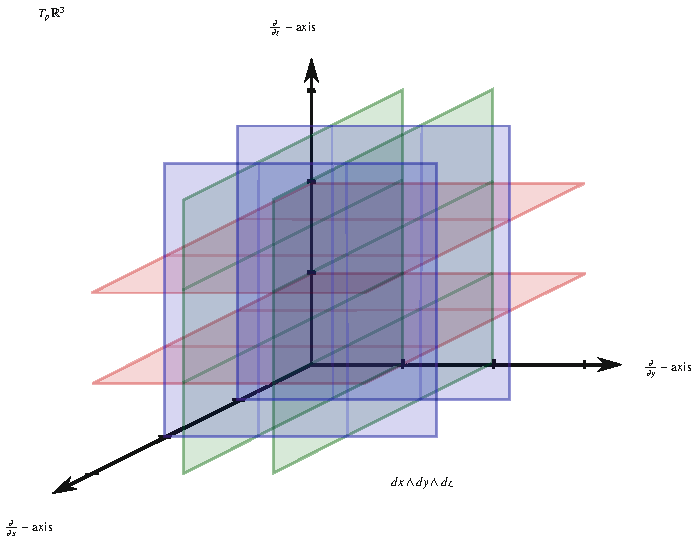
\includegraphics[width=0.960\linewidth]{images/vector/fig-5-30.pdf}
  \caption{三形式 $dx\wedge dy\wedge dz$ 由"立方体"组成，这些立方体的面是垂直于 $x$ 轴、$y$ 轴与 $z$ 轴的平面}
  \label{fig:5-30}
\end{figure}

\begin{question}\label{q:5-20}
基于图~\ref{fig:5-30}，为三形式 $2dx\wedge dy\wedge dz$ 画出三幅不同的草图.
\end{question}

\begin{question}\label{q:5-21}
设
\[
u=\begin{bmatrix}1\\0\\0\end{bmatrix},\qquad
v=\begin{bmatrix}0\\1\\0\end{bmatrix},\qquad
w=\begin{bmatrix}0\\0\\1\end{bmatrix}.
\]
在 $u$、$v$、$w$ 的不同排列上求值 $dx\wedge dy\wedge dz$，并用你的答案确定 $dx\wedge dy\wedge dz$ 具有什么样的定向. （注意，三个方向都必须以某种方式被考虑进去.）
\end{question}

\begin{question}\label{q:5-22}
你如何描绘图~\ref{fig:5-30} 中 $dx\wedge dy\wedge dz$ 的正定向？负定向呢？
\end{question}

\section{流形上形式的图形}

到目前为止我们一直在做的是，尝试画出 $\mathbb{R}^2$ 上的一形式与二形式以及 $\mathbb{R}^3$ 上的一形式、二形式与三形式的图形表示. 在每种情形下，我们都在点 $p$ 处考察某个形式 $\alpha_p$，并在点 $p$ 处的切空间中找到 $\alpha_p$ 的一个表示. 对 $\mathbb{R}^2$ 上的一形式，我们的图是 $T_p\mathbb{R}^2$ 中的直线（图~\ref{fig:5-1}--\ref{fig:5-7}）；而对 $\mathbb{R}^2$ 上的二形式，我们的图是 $T_p\mathbb{R}^2$ 中的方框（图~\ref{fig:5-8}--\ref{fig:5-10}）. 对 $\mathbb{R}^3$ 中的一形式，我们的图是 $T_p\mathbb{R}^3$ 中的平面（图~\ref{fig:5-11}--\ref{fig:5-18}）；对 $\mathbb{R}^3$ 中的二形式，我们的图是 $T_p\mathbb{R}^3$ 中的管子（图~\ref{fig:5-19}--\ref{fig:5-29}）；对 $\mathbb{R}^3$ 中的三形式，我们的图是 $T_p\mathbb{R}^3$ 中的立方体（图~\ref{fig:5-30}）.

有时人们会尝试利用这些 $\mathbb{R}^2$ 上的一形式与二形式以及 $\mathbb{R}^3$ 上的一形式、二形式与三形式的图形表示来"画出"整个流形上的形式，至少对二维或三维的流形是如此. 这通常有两种做法. 第一种方法至少在数学上说得通，尽管在某种意义上它仍可能是不完整的，并可能错误地表示微分形式. 不幸的是，第二种方法除可能错误地表示微分形式外，还有一些严重的数学缺陷. 但当这些方法确实可行时，它们可以成为思考二维与三维流形上微分形式的一种极其有用而富有启发的途径. 最好在脑海中记住，这些方法给出的图充其量只是漫画.

首先，我们介绍在流形上可视化形式的第一种方法. 这里所做的基本上是：在流形上选取一个点阵 $p_{ij}=(x_i,y_j)$，并在每个这样的阵点上把表示 $T_{p_{ij}}M$ 中一形式的线桩画在流形上. 图~\ref{fig:5-31} 显示了如何对 $\mathbb{R}^2$ 上一系列简单的一形式做到这一点. 箭头指向表示正方向. 当然，我们可以选择流形上密度不同的点阵. 图~\ref{fig:5-32} 用两种不同的点阵显示了 $\mathbb{R}^2$ 上相同的一形式 $xdx+ydy$. 二形式将类似，只是在每个点画一个小方框网格. 这种方法的缺点是点阵的间距；如果选择了不合适的点阵，完全有可能漏掉微分形式的重要细节. 尽管如此，人们通常仍会得到一个合理的漫画，它至少可以帮助人们想象这个微分形式.

\begin{figure}[htbp]
  \centering
  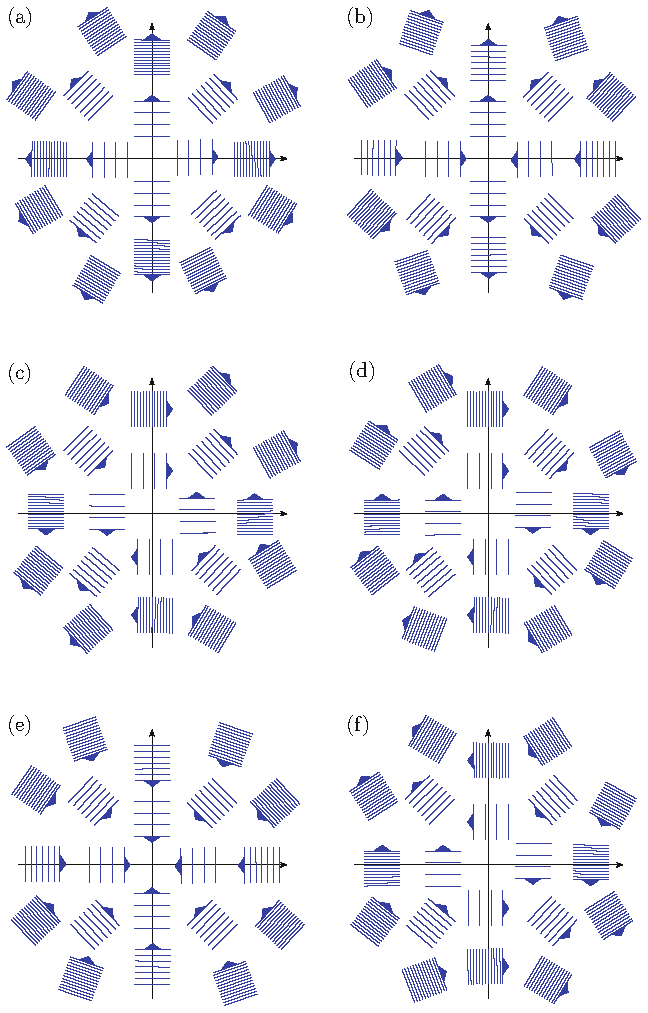
\includegraphics[width=0.768\linewidth]{images/vector/fig-5-31.pdf}
  \caption{流形 $\mathbb{R}^2$ 上的一形式，表示为流形 $\mathbb{R}^2$ 上的线桩网格. 箭头指向表示正方向（图像由 Vector Field Analyzer II, Version 2, Kawski, 2001 生成）. (a) $xdx+ydy$. (b) $-xdx+ydy$. (c) $ydx+xdy$. (d) $ydx-xdy$. (e) $-xdx-ydy$. (f) $-ydx-xdy$}
  \label{fig:5-31}
\end{figure}

对三维流形，图形是类似的. 首先在流形上选取一个三维点阵 $p_{ijk}=(x_i,y_j,z_k)$. 那么一形式将在每个点 $p_{ijk}$ 处表示为小的薄片桩，二形式将在每个点 $p_{ijk}$ 处表示为小的管子束，三形式将在每个点 $p_{ijk}$ 处表示为小的一组立方体.

\begin{figure}[htbp]
  \centering
  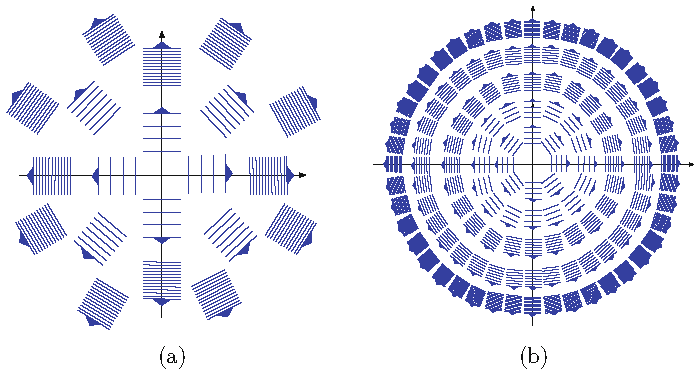
\includegraphics[width=0.830\linewidth]{images/vector/fig-5-32.pdf}
  \caption{流形 $\mathbb{R}^2$ 上的一形式 $xdx+ydy$，用两种不同的点阵表示为线桩网格. 箭头指向表示正方向. 注意右图中的线桩在中部开始看起来像是融合成同心圆（图像由 Vector Field Analyzer II, Version 2, Kawski, 2001 生成）}
  \label{fig:5-32}
\end{figure}

第二种方法做了类似的事情，但试图更进一步. 再次考虑图~\ref{fig:5-32}. 在第二幅图像中，点阵取得足够密，以至于特别是在中部，它们开始相互融合并形成同心圆. 在第二种方法中，阵点处的小图被相互连接起来，以在流形上提供一幅连续的图像. 当这确实可行时，这些图像是非常吸引人且容易思考的. 我们首先看看方法二在合适的时候是如何工作的，然后简要讨论方法二在一般情况下是如何失败的.

作为例子，图~\ref{fig:5-33} 在 $\mathbb{R}^2$ 上显示了一个一般的一形式 $\alpha$. 这里，阵点（未显示）处的线桩被尽可能好地连接起来，以生成覆盖流形的曲线. $\alpha(v)$ 的值（近似地）由向量 $v$ 刺穿的曲线条数给出. 流形 $\mathbb{R}^2$ 上二形式的情形被完全相同地处理，只是不是在每个阵点处画小的线桩，而是有小的方框补丁. 同样，有可能把这些方框连接起来，给出流形上二形式的粗略图像. 考虑图~\ref{fig:5-34}. 这里，流形 $\mathbb{R}^2$ 上的一个二形式被描绘在流形 $\mathbb{R}^2$ 上. 为了求出二形式 $\alpha$ 在任意给定点 $p$ 处的值，需要给出该点处的两个向量 $v_1$ 与 $v_2$. 那么 $\alpha_p(v_1,v_2)$ 的值由 $v_1$ 与 $v_2$ 张成的平行六面体内部的方框个数给出.

\begin{figure}[htbp]
  \centering
  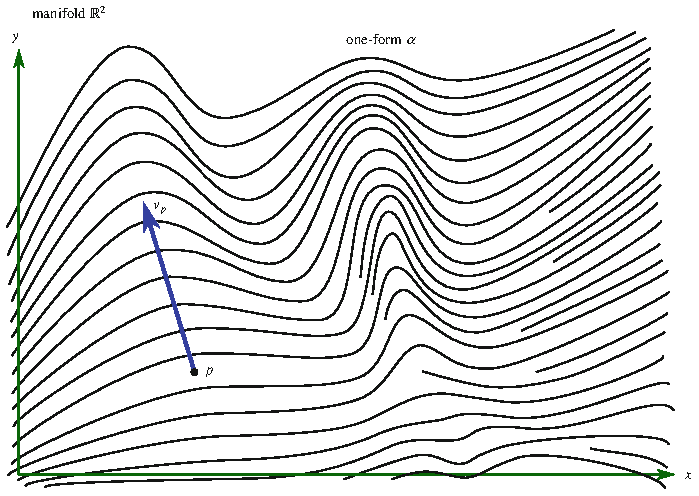
\includegraphics[width=0.876\linewidth]{images/vector/fig-5-33.pdf}
  \caption{流形 $\mathbb{R}^2$ 上展示了一个一形式 $\alpha$，所有"线桩"都被平滑地连接成曲线. 一形式作用在向量上的值（近似地）等于该向量"刺穿"的曲线的条数. 这里，$\alpha(v_p)\approx6$}
  \label{fig:5-33}
\end{figure}

在流形 $\mathbb{R}^3$ 上描绘一形式、二形式与三形式的尝试非常类似. 同样，选取一个点阵 $p_{ijk}=(x_i,y_j,z_k)$，并在每个这样的点处找到 $T_{p_{ijk}}\mathbb{R}^3$ 中该形式的图. 对在每个点 $p_{ijk}$ 处的一形式 $\alpha$，将有一桩二维薄片，类似于图~\ref{fig:5-17}. 然后，这些图中的每一幅的小副本将被叠加在每个阵点处的流形 $\mathbb{R}^3$ 上. 然后人们会尽可能好地尝试把这些薄片连接起来，得到一幅类似于图~\ref{fig:5-35} 的图. 薄片的紧密程度（换句话说，薄片彼此相隔多远）由特定的这个一形式决定. 为了求出 $\alpha(v)$ 的（近似）值，人们将数出向量 $v$ 刺穿的薄片张数. 所以，一形式 $10\alpha$ 的薄片彼此相距的距离是一形式 $\alpha$ 的薄片的十分之一.

\begin{figure}[htbp]
  \centering
  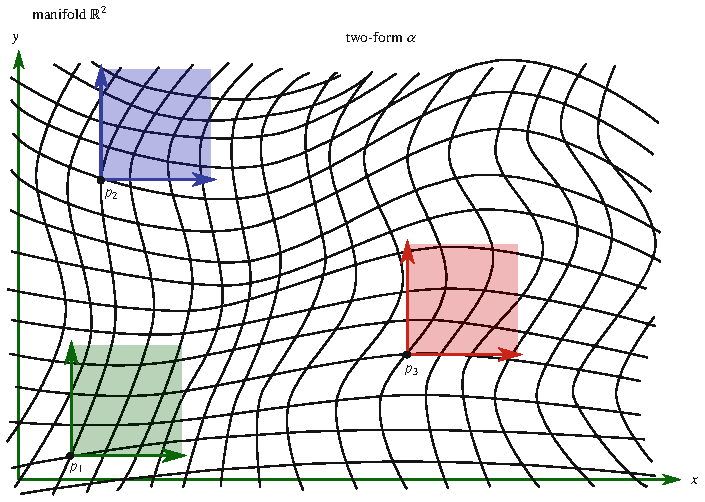
\includegraphics[width=0.875\linewidth]{images/vector/fig-5-34.pdf}
  \caption{流形 $\mathbb{R}^2$ 上展示了一个二形式 $\alpha$，所有方框都被平滑地连接起来. 单位向量 $e_1$ 与 $e_2$ 被描绘在点 $p_1$（绿）、$p_2$（蓝）与 $p_3$（红）处. 通过数出落在 $e_1$ 与 $e_2$ 在每个点处张成的平行六面体范围内的方框个数，可以（近似地）求出 $\alpha_{p_i}(e_1,e_2)$. 因此 $\alpha_{p_1}(e_1,e_2)\approx12$、$\alpha_{p_2}(e_1,e_2)\approx16$、$\alpha_{p_3}(e_1,e_2)\approx9$. 显然，虽然这是一幅漂亮的图，但它给出的答案只是非常近似的}
  \label{fig:5-34}
\end{figure}

对在每个点 $p_{ijk}$ 处的二形式 $\alpha$，将有一束"管子"，类似于图~\ref{fig:5-23}. 在每个阵点处，管子束的密度会变化，方向也会不同. 然后人们会尽可能好地尝试把这些薄片连接起来，得到一幅类似于图~\ref{fig:5-36} 的图，其中大小不同的管子蜿蜒穿过 $\mathbb{R}^3$. 管子排列的密度取决于二形式 $\alpha$ 的确切性质. 为了（近似地）求出 $\alpha(v_p,w_p)$，人们找到由 $v_p$ 与 $w_p$ 张成的平行六面体，并数出穿过这个平行六面体的管子根数.

\begin{figure}[htbp]
  \centering
  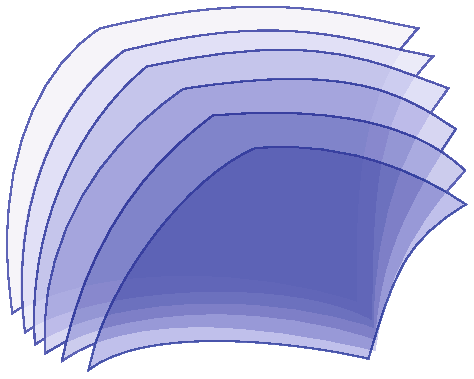
\includegraphics[width=0.656\linewidth]{images/vector/fig-5-35.pdf}
  \caption{$\mathbb{R}^3$ 中一个一般的一形式由填满 $\mathbb{R}^3$ 的薄片组成}
  \label{fig:5-35}
\end{figure}

对在每个点 $p_{ijk}$ 处的三形式 $\alpha$，将有一小组立方体，类似于图~\ref{fig:5-30}. 人们可以想象在每个阵点处有大小与方向各异的魔方. 然后这些立方体被尽可能好地全部连接起来，用小的立方体填满 $\mathbb{R}^3$. 我们在这里不再试图展示这一点. 求出 $\alpha(u_p,v_p,w_p)$ 的（近似）值归结为数出由 $u_p$、$v_p$、$w_p$ 张成的平行六面体内部的立方体个数.

\begin{figure}[htbp]
  \centering
  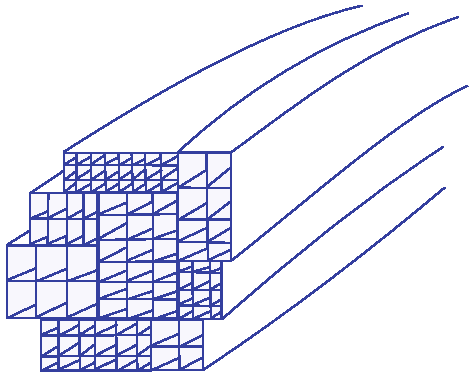
\includegraphics[width=0.657\linewidth]{images/vector/fig-5-36.pdf}
  \caption{$\mathbb{R}^3$ 中一个一般的二形式由填满 $\mathbb{R}^3$ 的管子组成}
  \label{fig:5-36}
\end{figure}

这种看待微分形式的方式有一些非常吸引人的地方，在某些情形下，它有助于提供一种在二维与三维流形上思考微分形式的额外方式. 不幸的是，在一般情况下方法二是失败的. 事实上，不用费多大力气就能找到方法二实际上无法可视化它们的形式的例子. 真正的问题之一是"连接"这件事. 从数学上看，这完全是障眼法，没有任何合理的理由. 事实上，一形式的每个线桩都位于不同的切空间中，所以"连接"线桩根本说不通. 而且，即使我们像上面那样在流形上画出这些图，也没有理由认为彼此靠近的阵点处的线桩会以允许它们被连接的方式定向，正如图~\ref{fig:5-32} 的情形那样. 对一般的一形式，它们不必如此. 当然，这也适用于三维流形的薄片桩与管子束.

一个必要但不充分的要求是，由微分形式的核给出的分布是可积的. 这将给出所谓的流形上的\newterm{foliation}{叶状结构}{foliation}，它允许线桩、薄片桩或管子束排列起来. 探索并解释这一点超出了本书的范围. 只需认识到，即使 $\mathbb{R}^3$ 上像 $xdy+dz$ 这样简单的一形式也无法使用方法二可视化.

然而，这种可视化微分形式的方式有时确实出现在物理学中. 物理学家并不太关心一种完全一般的可视化形式的方式，他们感兴趣的是对正在处理的物理问题与物理情形有效的可视化方式. 因此，这种方法在特定情形下确实有一些用处. 在合适的时候，它确实提供了一种非常好的思考形式的方式. 事实上，它为 Stokes 定理提供了一幅很好的配图，非常吸引人，将在第 11.6 节给出.

\section{Hodge 星算子可视化导引}

此时以数学上严谨的方式引入 Hodge 星算子有点棘手，因为许多必要的数学尚未引入，然而与本章相伴随的 Hodge 星算子的几何图确实相当漂亮且容易理解，所以现在是做这件事的自然时机. 因此我们将试图取得平衡，提供图背后的一些数学，但不足以让你被理论细节压垮. 眼下我们将限于三维的情形，并给出合理性论证而不是严谨的证明.

首先我们考虑下列向量空间
\begin{align*}
\bigwedge_p^0(\mathbb{R}^3)=\operatorname{span}\{1\}, \\
\bigwedge_p^1(\mathbb{R}^3)=\operatorname{span}\{dx,dy,dz\}=T_p^*\mathbb{R}^3, \\
\bigwedge_p^2(\mathbb{R}^3)=\operatorname{span}\{dx\wedge dy,dy\wedge dz,dz\wedge dx\}, \\
\bigwedge_p^3(\mathbb{R}^3)=\operatorname{span}\{dx\wedge dy\wedge dz\},
\end{align*}
它们的维数分别是一、三、三与一. 这些空间中的每一个都定义有所谓的\newterm{inner-product}{内积}{inner product}. 此时我们不去为一个严谨的定义而分心，只简单地说，本质上，向量空间上的内积把每一对向量与一个实数联系起来. 话虽如此，我们要做的是解释 $\bigwedge_p^1(\mathbb{R}^3)$ 与 $\bigwedge_p^2(\mathbb{R}^3)$ 上的内积，即我们最感兴趣的两个空间. 我们从空间 $\bigwedge_p^1(\mathbb{R}^3)$ 开始. $\bigwedge_p^1(\mathbb{R}^3)$ 上的内积由矩阵
\[
\begin{bmatrix}
1 & 0 & 0\\
0 & 1 & 0\\
0 & 0 & 1
\end{bmatrix}
\]
给出. 但这是如何工作的呢？假设我们有两个一形式元素 $\alpha,\beta\in\bigwedge_p^1(\mathbb{R}^3)$. 我们可以把这些元素按基元素写成余向量
\begin{align*}
\alpha=adx+bdy+cdz=[a,b,c], \\
\beta=rdx+sdy+tdz=[r,s,t].
\end{align*}
那么 $\alpha$ 与 $\beta$ 的内积，一般记为 $\langle\alpha,\beta\rangle$，由
\[
\langle\alpha,\beta\rangle=\langle[a,b,c],[r,s,t]\rangle
\equiv[a,b,c]
\begin{bmatrix}
1 & 0 & 0\\
0 & 1 & 0\\
0 & 0 & 1
\end{bmatrix}
[r,s,t]^T
\]
给出，即
\[
=[a,b,c]\begin{bmatrix}r\\s\\t\end{bmatrix}
=ar+bs+ct.
\]

我们花一点时间指出，用尖括号 $\langle\cdot,\cdot\rangle$ 表示内积是标准记号，它与我们前面用来表示微分形式与向量之间的典范配对 $\langle\cdot,\cdot\rangle$ 是完全不同的东西. 你必须仔细观察尖括号里面是什么，才能知道它们代表什么. 另外，注意我们隐含地假定基元素有一个顺序，$dx$ 第一，$dy$ 第二，$dz$ 第三. 只有知道了这个顺序，我们才知道如何写出表示内积的矩阵.

类似地，我们将用相同的矩阵
\[
\begin{bmatrix}
1 & 0 & 0\\
0 & 1 & 0\\
0 & 0 & 1
\end{bmatrix}
\]
定义 $\bigwedge_p^2(\mathbb{R}^3)$ 上的内积，它以完全相同的方式工作. 因此如果我们有
\begin{align*}
\eta=adx\wedge dy+bdy\wedge dz+cdz\wedge dx=[a,b,c], \\
\xi=rdx\wedge dy+sdy\wedge dz+tdz\wedge dx=[r,s,t],
\end{align*}
那么 $\eta$ 与 $\xi$ 的内积，记为 $\langle\eta,\xi\rangle$，由
\[
\langle\eta,\xi\rangle=\langle[a,b,c],[r,s,t]\rangle
\equiv[a,b,c]
\begin{bmatrix}
1 & 0 & 0\\
0 & 1 & 0\\
0 & 0 & 1
\end{bmatrix}
[r,s,t]^T
\]
给出，即
\[
=[a,b,c]\begin{bmatrix}r\\s\\t\end{bmatrix}
=ar+bs+ct.
\]
同样，我们隐含地假定基有一个顺序，这样我们才会知道如何写出矩阵.

现在我们有了真正定义 Hodge 星算子所必需的构件，它也被称为 Hodge 星对偶算子. Hodge 星算子是一个同构（或映射）$\ast:\bigwedge_p^k(\mathbb{R}^n)\to\bigwedge_p^{n-k}(\mathbb{R}^n)$，它把 $k$-形式送到 $(n-k)$-形式. 那么这个同构是如何定义的呢？对每个 $k$-形式 $\alpha$，存在唯一的一个 $(n-k)$-形式 $\ast\alpha$，使得对任意 $(n-k)$-形式 $\beta$ 都有
\begin{center}
\fbox{\parbox{0.88\textwidth}{\centering
Hodge 星算子：$\alpha\wedge\beta=\langle\ast\alpha,\beta\rangle\sigma$，对任意 $\beta$ 成立
}}
\end{center}
其中 $\langle\cdot,\cdot\rangle$ 表示 $\bigwedge_p^{n-k}(\mathbb{R}^n)$ 上的内积，$\sigma$ 是 $n$ 维体积形式. 所以，$\ast\alpha$ 是根据这个相当复杂的关系来定义的. 我们想把这一关系展开，看看它试图表达什么，
\[
\underbrace{\underbrace{\alpha}_{k\text{-形式}}\wedge\underbrace{\beta}_{(n-k)\text{-形式}}}_{\text{一个 }n\text{-形式}}
=
\langle\underbrace{\ast\alpha}_{(n-k)\text{-形式}},\underbrace{\beta}_{(n-k)\text{-形式}}\rangle
\underbrace{\sigma}_{\text{体积形式（一个 }n\text{-形式）}}.
\]

所以我们在等式的左边与右边各得到一个 $n$-形式. 回忆体积形式 $\sigma$ 是已知的，$\alpha$ 是给定的，而 $\beta$ 可以是任意 $(n-k)$-形式. 然后我们利用这个关系找出 $\ast\alpha$ 是哪一个 $(n-k)$-形式. 由于 $\beta$ 可以是任意 $(n-k)$-形式，这意味着无论选择哪一个 $(n-k)$-形式作为 $\beta$，我们总是找到完全相同的 $\ast\alpha$. 在某种意义上，这是相当惊人的. 但映射 $\ast$ 是唯一的，这一事实我们在这里不试图证明，所以无论选择哪一个 $(n-k)$-形式作为 $\beta$，都只有一个 $\ast\alpha$.

现在，让我们把这个关系真正用在我们三维的情形. 我们首先看映射 $\ast:\bigwedge_p^1(\mathbb{R}^3)\to\bigwedge_p^2(\mathbb{R}^3)$. 首先我们着手求 $\ast dx$. 由于我们知道 $\ast dx$ 是一个二形式，我们知道它必有形式
\[
\ast dx=a\,dx\wedge dy+b\,dy\wedge dz+c\,dz\wedge dx=[a,b,c]
\]
对某三个数 $a,b,c$. 我们的目标是用关系
\[
dx\wedge\beta=\langle\ast dx,\beta\rangle\,dx\wedge dy\wedge dz
\]
求出 $a$、$b$、$c$ 是什么. 眼下我们考虑由
\[
\beta=r\,dx\wedge dy+s\,dy\wedge dz+t\,dz\wedge dx=[r,s,t]
\]
给出的一般二形式 $\beta$. 所以我们的定义关系变成
\begin{align*}
& dx\wedge(r\,dx\wedge dy+s\,dy\wedge dz+t\,dz\wedge dx) \\
&=\langle\ast dx,r\,dx\wedge dy+s\,dy\wedge dz+t\,dz\wedge dx\rangle\,dx\wedge dy\wedge dz \\
&=\langle[a,b,c],[r,s,t]\rangle\,dx\wedge dy\wedge dz \\
&=(ar+bs+ct)\,dx\wedge dy\wedge dz.
\end{align*}
在左边我们有
\begin{align*}
dx\wedge(r\,dx\wedge dy+s\,dy\wedge dz+t\,dz\wedge dx)
=r\underbrace{dx\wedge dx\wedge dy}_{=0}+s\,dx\wedge dy\wedge dz+t\underbrace{dx\wedge dz\wedge dx}_{=0} \\
=s\,dx\wedge dy\wedge dz.
\end{align*}
合并起来我们有
\[
s\,dx\wedge dy\wedge dz=(ar+bs+ct)\,dx\wedge dy\wedge dz,
\]
这给出
\[
s=ar+bs+ct.
\]
由于我们的定义关系无论选择哪个 $\beta$ 都成立，如果我们选择满足 $r=1$、$s=0$、$t=0$ 的 $\beta$，这个等式会给出 $a=0$. 如果我们选择满足 $r=0$、$s=1$、$t=0$ 的 $\beta$，这个等式会给出 $b=1$. 如果我们选择满足 $r=0$、$s=0$、$t=1$ 的 $\beta$，这个等式会给出 $c=0$. 因此我们得到
\[
\ast dx=dy\wedge dz.
\]
$dx$ 与 $\ast dx$ 之间的关系在图~\ref{fig:5-37} 中以图形方式显示. $\ast dx=dy\wedge dz$ 的管子垂直于 $dx$ 的平面.

\begin{figure}[htbp]
  \centering
  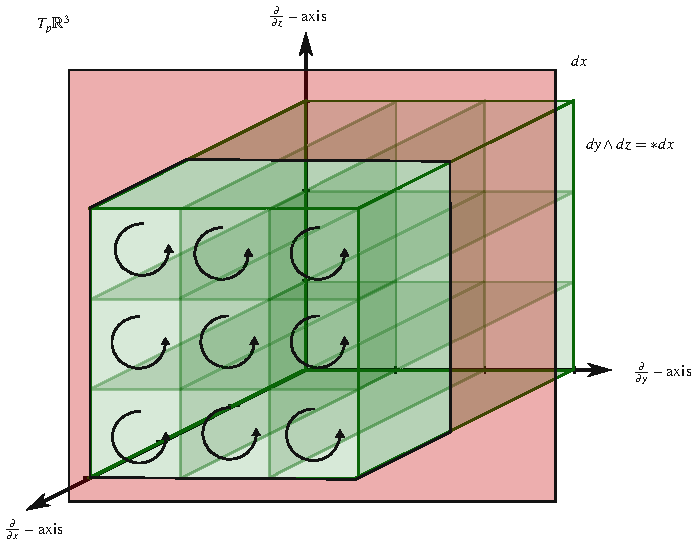
\includegraphics[width=0.828\linewidth]{images/vector/fig-5-37.pdf}
  \caption{$\ast dx$ 的管子垂直于 $dx$ 的平面. 即 $\ast dx=dy\wedge dz$}
  \label{fig:5-37}
\end{figure}

\begin{question}\label{q:5-23}
对下列 $\beta$ 证明 $dx\wedge\beta=\langle\ast dx,\beta\rangle\,dx\wedge dy\wedge dz$：
\begin{enumerate}
  \item[(a)] $\beta=7dx\wedge dy-3dy\wedge dz+2dz\wedge dx$，
  \item[(b)] $\beta=20dx\wedge dy+15dy\wedge dz-10dz\wedge dx$，
  \item[(c)] $\beta=-4dx\wedge dy-6dy\wedge dz-8dz\wedge dx$.
\end{enumerate}
\end{question}

我们将重做这个计算来求 $\ast dy$. 和以前一样，由于我们知道 $\ast dy$ 是一个二形式，我们知道它必有形式
\[
\ast dy=a\,dx\wedge dy+b\,dy\wedge dz+c\,dz\wedge dx=[a,b,c]
\]
对某三个数 $a,b,c$，并且我们希望用关系
\[
dy\wedge\beta=\langle\ast dy,\beta\rangle\,dx\wedge dy\wedge dz
\]
求出 $a$、$b$、$c$ 是什么. 同样，我们假设
\[
\beta=r\,dx\wedge dy+s\,dy\wedge dz+t\,dz\wedge dx=[r,s,t],
\]
结果得到
\begin{align*}
& dy\wedge(r\,dx\wedge dy+s\,dy\wedge dz+t\,dz\wedge dx) \\
&=\langle\ast dy,r\,dx\wedge dy+s\,dy\wedge dz+t\,dz\wedge dx\rangle\,dx\wedge dy\wedge dz \\
&=(ar+bs+ct)\,dx\wedge dy\wedge dz.
\end{align*}
左边变成
\begin{align*}
dy\wedge(r\,dx\wedge dy+s\,dy\wedge dz+t\,dz\wedge dx)
=r\underbrace{dy\wedge dx\wedge dy}_{=0}+s\underbrace{dy\wedge dy\wedge dz}_{=0}+t\,dy\wedge dz\wedge dx \\
=t\,dx\wedge dy\wedge dz.
\end{align*}
合并起来我们有
\[
t\,dx\wedge dy\wedge dz=(ar+bs+ct)\,dx\wedge dy\wedge dz,
\]
这给出
\[
t=ar+bs+ct.
\]
由于我们的定义关系无论选择哪个 $\beta$ 都成立，如果我们选择满足 $r=1$、$s=0$、$t=0$ 的 $\beta$，我们会得到 $a=0$. 如果我们选择满足 $r=0$、$s=1$、$t=0$ 的 $\beta$，我们会得到 $b=0$. 如果我们选择满足 $r=0$、$s=0$、$t=1$ 的 $\beta$，我们会得到 $c=1$. 因此我们会得到
\[
\ast dy=dz\wedge dx.
\]
再次注意，$\ast dy$ 的管子垂直于 $dy$ 的平面. 见图~\ref{fig:5-38}.

\begin{figure}[htbp]
  \centering
  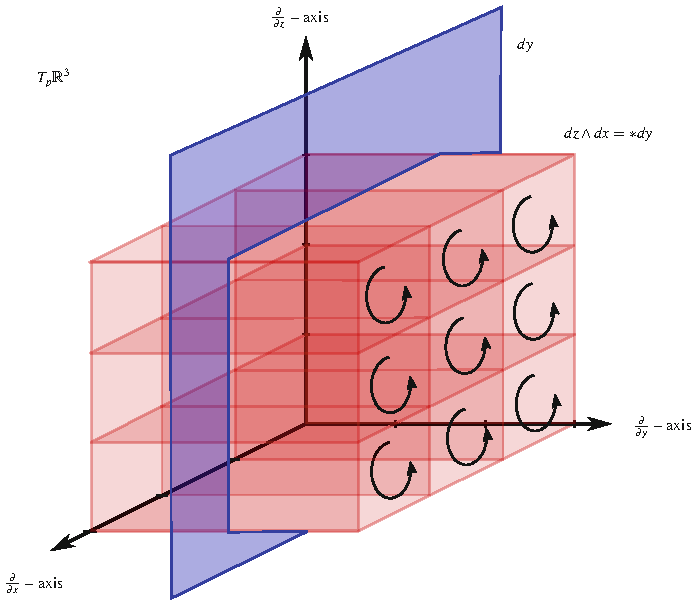
\includegraphics[width=0.830\linewidth]{images/vector/fig-5-38.pdf}
  \caption{$\ast dy$ 的管子垂直于 $dy$ 的平面. 即 $\ast dy=dz\wedge dx$}
  \label{fig:5-38}
\end{figure}

\begin{question}\label{q:5-24}
对下列 $\beta$ 证明 $dy\wedge\beta=\langle\ast dy,\beta\rangle\,dx\wedge dy\wedge dz$：
\begin{enumerate}
  \item[(a)] $\beta=7dx\wedge dy-3dy\wedge dz+2dz\wedge dx$，
  \item[(b)] $\beta=20dx\wedge dy+15dy\wedge dz-10dz\wedge dx$，
  \item[(c)] $\beta=-4dx\wedge dy-6dy\wedge dz-8dz\wedge dx$.
\end{enumerate}
\end{question}

\begin{question}\label{q:5-25}
利用定义恒等式 $dz\wedge\beta=\langle\ast dz,\beta\rangle\,dx\wedge dy\wedge dz$（对所有 $\beta\in\bigwedge_p^2(\mathbb{R}^3)$）求 $\ast dz$.
\end{question}

与 $\ast dz$ 相联系的图像显示 $\ast dz$ 的管子垂直于 $dz$ 的平面，见图~\ref{fig:5-39}.

\begin{figure}[htbp]
  \centering
  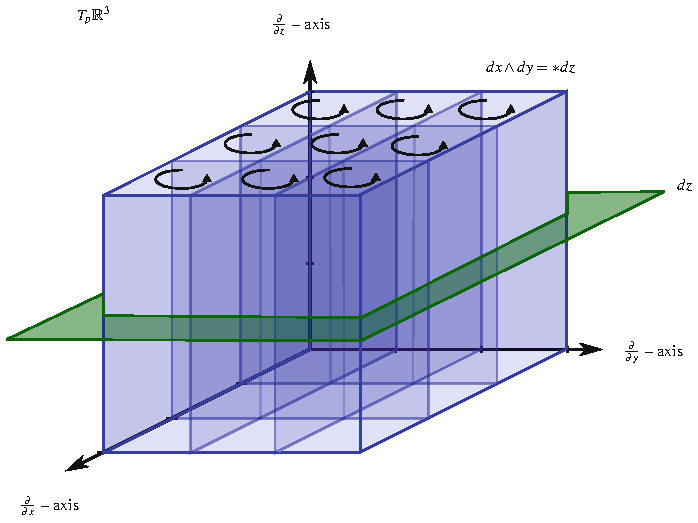
\includegraphics[width=0.827\linewidth]{images/vector/fig-5-39.pdf}
  \caption{$\ast dz$ 的管子垂直于 $dz$ 的平面. 即 $\ast dz=dx\wedge dy$}
  \label{fig:5-39}
\end{figure}

\begin{question}\label{q:5-26}
对下列 $\beta$ 证明 $dz\wedge\beta=\langle\ast dz,\beta\rangle\,dx\wedge dy\wedge dz$：
\begin{enumerate}
  \item[(a)] $\beta=7dx\wedge dy-3dy\wedge dz+2dz\wedge dx$，
  \item[(b)] $\beta=20dx\wedge dy+15dy\wedge dz-10dz\wedge dx$，
  \item[(c)] $\beta=-4dx\wedge dy-6dy\wedge dz-8dz\wedge dx$.
\end{enumerate}
\end{question}

\begin{question}\label{q:5-27}
利用 Hodge 星算子的定义求 $*(dx\wedge dy)$、$*(dy\wedge dz)$ 与 $*(dz\wedge dx)$.
\end{question}

\begin{question}\label{q:5-28}
你有时会看到 Hodge 星算子的另一种定义. 由于这是一个处理起来稍微容易的定义，我们把它留作练习. 证明 Hodge 星算子的这个替代定义
\[
\alpha\wedge\ast\beta=\langle\alpha,\beta\rangle\sigma,\qquad\text{对任意 }\alpha
\]
对 $*dx$、$*dy$、$*dz$、$*(dx\wedge dy)$、$*(dy\wedge dz)$、$*(dz\wedge dx)$ 给出相同的值.
\end{question}

现在我们来看 $\mathbb{R}^4$ 上形式的 Hodge 星对偶算子. 在四维中，试图画图要困难得多，但数学计算是相当直接的. 首先我们定义记号与我们的空间. 我们将用 $x_1,x_2,x_3,x_4$ 作为我们的笛卡尔坐标函数. 在 $\mathbb{R}^3$ 中循环书写以保持整洁很管用，但在 $\mathbb{R}^4$ 中就没有那么有用了，所以我们不再这样做. 这里的约定是使用递增顺序. 我们将使用的空间是
\begin{align*}
\bigwedge^0(\mathbb{R}^4)=C(\mathbb{R}^4)=\mathbb{R}^4\text{ 上的函数}, \\
\bigwedge^1(\mathbb{R}^4)=\operatorname{Span}\{dx_1,dx_2,dx_3,dx_4\}, \\
\bigwedge^2(\mathbb{R}^4)=\operatorname{Span}\{dx_1\wedge dx_2,dx_1\wedge dx_3,dx_1\wedge dx_4,dx_2\wedge dx_3,dx_2\wedge dx_4,dx_3\wedge dx_4\}, \\
\bigwedge^3(\mathbb{R}^4)=\operatorname{Span}\{dx_1\wedge dx_2\wedge dx_3,dx_1\wedge dx_2\wedge dx_4,dx_1\wedge dx_3\wedge dx_4,dx_2\wedge dx_3\wedge dx_4\}, \\
\bigwedge^4(\mathbb{R}^4)=\operatorname{Span}\{dx_1\wedge dx_2\wedge dx_3\wedge dx_4\}.
\end{align*}
这些空间上的内积（Hodge 星对偶定义右边所必需的）由单位矩阵给出. 目前我们对此不作过多追究，但流形的度量（内积正是由它导出的）我们将在第 A.6 节更详细地讨论.

现在我们利用问题~\ref{q:5-28} 中给出的 Hodge 星对偶的定义求一个一形式基元素的 Hodge 星对偶，
\begin{align*}
dx_1\wedge\ast dx_1=\underbrace{\langle dx_1,dx_1\rangle}_{=1}\,dx_1\wedge dx_2\wedge dx_3\wedge dx_4 \\
\Longrightarrow\ \ast dx_1=dx_2\wedge dx_3\wedge dx_4.
\end{align*}
注意，通过把 $dx_1$ 与 $\ast dx_1$ 楔起来，我们得以在等式右边利用 $\bigwedge^1(\mathbb{R}^4)$ 上内积的优良性质，在那里我们有 $\langle dx_1,dx_1\rangle=1$. 求二形式基元素的 Hodge 星对偶类似：
\begin{align*}
(dx_1\wedge dx_2)\wedge\ast(dx_1\wedge dx_2)=\underbrace{\langle dx_1\wedge dx_2,dx_1\wedge dx_2\rangle}_{=1}\,dx_1\wedge dx_2\wedge dx_3\wedge dx_4 \\
\Longrightarrow\ \ast(dx_1\wedge dx_2)=dx_3\wedge dx_4.
\end{align*}

\begin{question}\label{q:5-29}
求 $\ast dx_2$、$\ast dx_3$、$\ast dx_4$.
\end{question}

\begin{question}\label{q:5-30}
求 $*(dx_1\wedge dx_3)$、$*(dx_1\wedge dx_4)$、$*(dx_2\wedge dx_3)$、$*(dx_2\wedge dx_4)$、$*(dx_3\wedge dx_4)$.
\end{question}

\begin{question}\label{q:5-31}
求 $*(dx_1\wedge dx_2\wedge dx_3)$、$*(dx_1\wedge dx_2\wedge dx_4)$、$*(dx_1\wedge dx_3\wedge dx_4)$、$*(dx_2\wedge dx_3\wedge dx_4)$.
\end{question}

\begin{question}\label{q:5-32}
求 $*(dx_1\wedge dx_2\wedge dx_3\wedge dx_4)$.
\end{question}

\section{小结、参考文献与问题}

\subsection{小结}

我们现在花一点时间用一些评论来结束本章. 如果你是数学专业的学生，你可能永远不会在你的任何教科书里看到这种描绘或表示微分形式的方式；我肯定从来没有. 然而，如果你是物理专业的学生，那么很有可能会看到以这种方式讨论或呈现微分形式，无论是在电磁学课程中，还是在相对论课程中. 这些图像在试图理解某些方程并描绘这些方程背后的物理现象时非常有用. 我们将在后续章节详细探讨其中的一些物理应用. 尽管这些图在描绘方程试图表达的意思方面能提供很大的帮助，但在实际计算中使用它们通常是困难的，而且不值得费力，因为它们只给出近似答案. 使用微分形式的计算规则来计算精确的数值答案，并使用这些图来辅助概念性的理解.

此外，人们可以发展这些图像的高维类似物. 例如，把时间考虑进去，从相对论之前的欧几里得视角来看待时空，就会得到它的一个四维版本. 在狭义相对论与广义相对论两种情形下把时间包括进来也会得到四维版本，但在这些情形下，由于流形上的度量（想想内积）不同，基于内积的 Hodge 星算子也会改变. 然而，维度越高，使用这些图就越困难，使用得也越少，尽管想象 1 维与 $n-1$ 维的情形通常仍然是够清楚的.

Hodge 星算子的两个等价定义如下给出，
\begin{center}
\fbox{\parbox{0.88\textwidth}{\centering
Hodge 星算子定义一：$\alpha\wedge\beta=\langle\ast\alpha,\beta\rangle\sigma$，对任意 $\beta$ 成立；\\
Hodge 星算子定义二：$\alpha\wedge\ast\beta=\langle\alpha,\beta\rangle\sigma$，对任意 $\alpha$ 成立
}}
\end{center}

\subsection{参考文献与进一步阅读}

本章的材料几乎只出现在物理学中. 这是有原因的——作为一种思考微分形式的严谨方式，它在几个方面有所欠缺. 关于这种在流形上可视化形式的方式及其欠缺之处的批评，见 Bachman~\cite{ref04}. 但作为一种在各类物理情形中相当宽松地思考微分形式的方式，它相当有用，并且从物理系统的角度来看可能相当富有启发性. 正如本章开头提到的，这部分材料的主要来源是 Misner、Thorne 和 Wheeler~\cite{ref34}，不过也使用了 Dray~\cite{ref16}、Warnick、Selfridge 和 Arnold~\cite{ref49}、Warnick 与 Russer~\cite{ref48} 以及 DesChamps~\cite{ref13}. 所有这些来源都属于物理学的领域. 事实上，最后三篇文献强烈主张把这些可视化微分形式的技术作为教授电磁学的教学工具，尽管我们不知道有任何相当完整的实际尝试. 唯一另一个试图沿着本章材料思路给出几何解释的真正数学来源是 Burke~\cite{ref08}，而他的目标读者同样是在职物理学家. 用于生成 $\mathbb{R}^2$ 中一形式的线桩图像的软件是 Kawski~\cite{ref28} 编写的 Vector Field Analyzer II，可在网上获得.

\subsection{问题}

\begin{question}\label{q:5-33}
画出 $\mathbb{R}^2$ 上的坐标函数 $z$，并求出坐标函数 $y$ 沿下列向量的"rise"：
\begin{enumerate}
  \item[(a)] $\binom{0}{1}$，即从点 $(0,0)$ 到点 $(0,1)$，
  \item[(b)] $\binom{1}{1}$，即从点 $(0,0)$ 到点 $(1,1)$，
  \item[(c)] $\binom{-1}{2}$，即从点 $(0,0)$ 到点 $(-1,2)$，
  \item[(d)] $\binom{2}{-3}$，即从点 $(0,0)$ 到点 $(2,-3)$.
\end{enumerate}
\end{question}

\begin{question}\label{q:5-34}
画出表示 $\mathbb{R}^2$ 上下列一形式的图：$7dx$、$-3dy$、$-\frac23dx$、$-\frac13dy$ 与 $\frac25dy$.
\end{question}

\begin{question}\label{q:5-35}
画出 $\mathbb{R}^2$ 上下列一形式的图形表示：$\frac12dx+2dy$、$-\frac13dx-\frac12dy$ 与 $-dx-\frac23dy$.
\end{question}

\begin{question}\label{q:5-36}
为下列每个二形式在 $\mathbb{R}^2$ 上画出三种图形表示：$5dx\wedge dy$、$\frac12dx-\frac12dy$ 与 $2dx+\frac23dy$.
\end{question}

\begin{question}\label{q:5-37}
在 $\mathbb{R}^3$ 上画出一形式 $dx-dy$、$-dx+dy$、$dy-dz$ 与 $-dx-dz$ 的草图.
\end{question}

\begin{question}\label{q:5-38}
为下列每个二形式在 $\mathbb{R}^3$ 上找出两种图形表示：$5dx\wedge dy$、$6dy\wedge dz$ 与 $\frac14dz\wedge dx$.
\end{question}

\begin{question}\label{q:5-39}
为下列每个二形式在 $\mathbb{R}^3$ 上画出一幅草图：$3dy\wedge dz+2dz\wedge dx$、$dx\wedge dy+3dz\wedge dx$ 与 $2dx\wedge dy+4dy\wedge dz+3dz\wedge dx$.
\end{question}

\begin{question}\label{q:5-40}
在 $\mathbb{R}^3$ 上画出二形式 $-dx\wedge dy+dy\wedge dz$、$dx\wedge dy-dy\wedge dz$ 与 $-dx\wedge dy-dy\wedge dz$ 的草图. 负号有什么影响？用一些精心选择的向量来帮助你弄清楚.
\end{question}

\begin{question}\label{q:5-41}
把下面的一形式与图~\ref{fig:5-40} 中描绘的图像配对：
\begin{enumerate}
  \item[(a)] $\sin(x)dx+ydy$，
  \item[(b)] $dx-dy$，
  \item[(c)] $xdx+\cos(y)dy$，
  \item[(d)] $\sin(x)dx+xdy$.
\end{enumerate}
\end{question}

\begin{figure}[htbp]
  \centering
  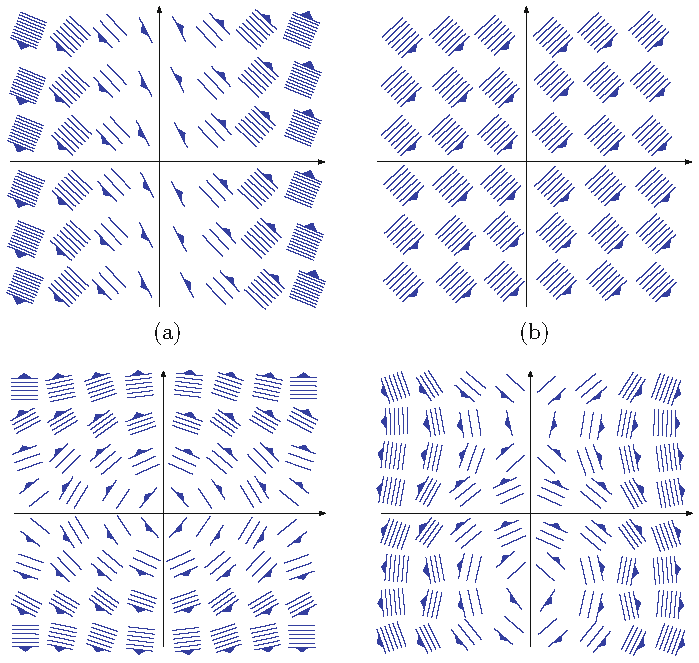
\includegraphics[width=0.829\linewidth]{images/vector/fig-5-40.pdf}
  \caption{问题~\ref{q:5-41} 的图像（图像由 Vector Field Analyzer II, Version 2, Kawski, 2001 生成）.}
  \label{fig:5-40}
\end{figure}

\begin{question}\label{q:5-42}
设流形是 $\mathbb{R}^4$. 求 $\ast dx_2$、$\ast dx_3$、$\ast dx_4$.
\end{question}

\begin{question}\label{q:5-43}
设流形是 $\mathbb{R}^4$. 求 $*(dx_1\wedge dx_3)$、$*(dx_1\wedge dx_4)$、$*(dx_2\wedge dx_3)$、$*(dx_2\wedge dx_4)$、$*(dx_3\wedge dx_4)$.
\end{question}

\begin{question}\label{q:5-44}
设流形是 $\mathbb{R}^4$. 求 $*(dx_1\wedge dx_2\wedge dx_3)$、$*(dx_1\wedge dx_2\wedge dx_4)$、$*(dx_1\wedge dx_3\wedge dx_4)$、$*(dx_2\wedge dx_3\wedge dx_4)$.
\end{question}

\begin{question}\label{q:5-45}
设流形是 $\mathbb{R}^4$. 求 $*(dx_1\wedge dx_2\wedge dx_3\wedge dx_4)$.
\end{question}
